%%%%%%%%%%%%%%%%%%%%% RJT TeX Template %%%%%%%%%%%%%%%%%%%%%
\documentclass[twoside,11pt,a4paper]{article}

%%%% BHAM PREAMBLE - SET THIS FIRST! %%%%
\newcommand{\bhamstudentname}{Sarathkumar Padinjare Marath Sankaranarayanan}
\newcommand{\bhamthesistitle}{Machine Learning \& Deep Learning Approaches to Predict Credit Card Default}
\newcommand{\bhamfronttitle}{Machine Learning \& Deep Learning Approaches \\ to Predict Credit Card Default}
\newcommand{\bhamschool}{School of Computer Science}
\newcommand{\bhamcollege}{Engineering and Physical Sciences}
\newcommand{\bhamdegree}{MSc. Artificial Intelligence \& Computer Science}
\newcommand{\bhamid}{2359859}
\newcommand{\bhamsupervisor}{Dr.Kashif Rajpoot}
\newcommand{\bhamyear}{2022}
%%%%           %%%%


\usepackage[hyphens]{url}
\usepackage[breaklinks,linktocpage]{hyperref}
\usepackage{fancyhdr}
\usepackage[sort]{natbib} 
\usepackage{comment} % from http://www.latex-community.org/forum/viewtopic.php?f=5&t=4538
\usepackage{dirtree} % from http://blog.plenz.com/2011-07/represent-directory-structures-in-latex.html
\usepackage{longtable} % from http://stackoverflow.com/questions/2896833/how-to-stretch-a-table-over-multiple-pages
\usepackage{algorithm}   
\usepackage{algorithmic}   %both algorithm* from http://hasini-gunasinghe.blogspot.co.uk/2014/02/presenting-algorithmsprotocols-in-neat.html

\renewcommand{\algorithmiccomment}[1]{#1} %http://tex.stackexchange.com/q1uestions/61861/algorithmic-package-for-loop-and-comment-at-the-same-line
\usepackage[printonlyused]{acronym}
\usepackage[table]{xcolor}
\usepackage{subcaption}
\usepackage{placeins}

\pagestyle{fancy}
\renewcommand{\sectionmark}[1]{\markboth{#1}{}}	%from tex.stackexchange.com/questions/111361

\lfoot{\bhamstudentname}
\cfoot{}
\rfoot{}
\fancyhfoffset[L]{0cm} %this fixes the right page number margin issue.
\newcommand{\HRule}{\rule{\linewidth}{0.5mm}}
\renewcommand{\headrulewidth}{0pt}
\newcommand{\tab}{\hspace*{1.25em}}
\newcommand{\minitab}{\hspace*{0.25em}}

%footnote stuff
\usepackage{perpage}
\MakePerPage{footnote} %the perpage package command
\renewcommand*{\thefootnote}{\fnsymbol{footnote}}

\lhead{}\chead{}\rhead{}
\setlength{\headheight}{28pt} %fixes the warnings about headheight being too small
\setlength{\headsep}{6pt}
\pdfoutput=1 % we are running PDFLaTeX
\usepackage[left=2.55cm,right=1.6cm,top=1.8cm,bottom=1.8cm]{geometry}
\usepackage{titling}	
\setlength{\droptitle}{-2.75cm}   % This is your set screw\\
\usepackage{titlesec}
\titleformat*{\section}{\normalsize	\bfseries}
\titleformat*{\subsection}{\small \bfseries}
\titleformat*{\subsubsection}{\footnotesize \bfseries}
%modifies the size of the gaps between the top of the title and bottom
% arguments {type}{left}{top}{bottom}
\titlespacing*{\section} {0pt}{3ex plus 1ex minus .2ex}{2ex plus .2ex}
\titlespacing*{\subsection} {0pt}{2.25ex plus 1ex minus .2ex}{0.75ex plus .2ex}
\titlespacing*{\subsubsection}{0pt}{2.ex plus 1ex minus .2ex}{0.5ex plus .2ex}

\setlength{\intextsep}{0pt} %from http://tex.stackexchange.com/questions/25828/how-to-remove-change-the-vertical-spacing-before-and-after-an-algorithm-environ

\usepackage[pdftex]{graphicx}
\graphicspath{ {figures/} }


\usepackage{enumitem}
\usepackage{pdfpages}
\usepackage{lastpage}
\usepackage{amsmath}
\usepackage{amsfonts}
\usepackage{amssymb}


\usepackage{epstopdf} %http://dirkraffel.com/2007/11/19/include-eps-files-in-latex/comment-page-2/

\usepackage{listings}
\lstset{
 basicstyle=\ttfamily,
  columns=fullflexible,
  keepspaces=true,
breaklines=true
} %from http://tex.stackexchange.com/questions/121601/automatically-wrap-the-text-in-verbatim

\newcommand{\todo}[1]{\textcolor{red}{TODO: #1}\PackageWarning{TODO:}{TODO found: #1!}} %from http://tex.stackexchange.com/questions/9796/how-to-add-todo-notes

\DeclareGraphicsExtensions{.jpg,.jpeg,.png,.ppm}
%%%%%%%%%%%%%%%%%%%%%  END of TEMPLATE %%%%%%%%%%%%%%%%%%%%%

\title{MSc. Project\\\bhamthesistitle}
\author{\textsf{\bhamstudentname {\textsf{}}}}

\date{}
\begin{document}

\pagenumbering{gobble} % fix at	 http://tex.stackexchange.com/questions/7355/how-to-suppress-page-number
% this came from http://en.wikibooks.org/wiki/LaTeX/Title_Creation and http://tex.stackexchange.com/questions/14778/error-with-hrule
\begin{titlepage}
\begin{center}
% this was from http://tex.stackexchange.com/questions/7219/how-to-vertically-center-two-images-next-to-each-other
\begin{minipage}{6in}
  \centering
  \raisebox{-0.5\height}{
\includegraphics[width=1.25in]{crest}}
  \hspace*{.2in}
  \raisebox{-0.5\height}{
\includegraphics[height=0.9375in]{uni}}
  \end{minipage}
  \\ [1.0cm]
\textsc{{\LARGE \bhamschool\\}College of \bhamcollege}\\[3.5cm]

\textsc{\Large MSc. Project}\\[0.5cm]

% Title
\HRule \\[0.4cm]
\begin{center}\Huge
\bhamfronttitle
\end{center}
\HRule \\[1.5cm]
% Team and Members

\begin{center}
Submitted in conformity with the requirements\\ for the degree of \bhamdegree\\
\bhamschool\\ University of Birmingham\\
\vspace{2cm}
\bhamstudentname \\
Student ID: \bhamid\\
Supervisor: \bhamsupervisor      
\end{center}
\vfill

% Bottom of the page
{\large September \bhamyear}

\end{center}
\end{titlepage}

\section*{\centering Abstract}	


% Taken from the MSc Thesis template, and edited for a PGT report
The material contained within this report has not previously been
submitted for a degree at the University of Birmingham or any other university.
The research reported within this report has been conducted by the author
unless indicated otherwise.\\
\\
\textbf{Keywords} Credit Card Default Prediction, Ensemble Learning

\vfill
\clearpage

\section*{\centering Declaration}
% Taken from the MSc Thesis template, and edited for a PGT report
The material contained within this report has not previously been
submitted for a degree at the University of Birmingham or any other university.
The research reported within this report has been conducted by the author
unless indicated otherwise.\\
\\
\textbf{Signed} Sarathkumar Padinjare Marath Sankaranarayanan 

\vfill
\clearpage
\begin{center}
\vspace*{\fill}
\begin{minipage}{6in}

%\centering \Large{``Most men who have really lived have had, in some share, their great adventure.\\This railway is mine."}\\{\normalsize{\textsc{James J. Hill}}, \emph{Railway Pioneer}} \vspace{2cm}

%\centering \Large{``Steam engines don't answer back.\\ You can belt them with a hammer and they say nowt."}\\{\normalsize{\textsc{Fred Dibnah}}, \emph{Steeplejack and Engineer}} \vspace{2cm}

\centering \Large{``You have to learn the rules of the game.\\ And then you have to play better than anyone else"}\\{\normalsize{\textsc{Albert Einstein}}}

  \end{minipage}
  \vspace*{\fill}
\end{center}


\clearpage
\maketitle
\vspace{-5.5em} %fixes distance between \maketitle and the TOC
\begingroup
    \fontsize{9pt}{11pt}\selectfont
\tableofcontents
\endgroup
\clearpage
\phantomsection
\section*{Table of Abbreviations}

\normalsize
\begin{acronym}[SCEPTICS] % Give the longest label here so that the list is nicely aligned
\acro{SVM} {Support Vector Machine}
\acro{ANN} {Artificial Neural Network}
\acro{GBDT} {Gradient Boosting Decision Tree}
\acro{GRU} {Gated Recurrent Unit}
\acro{LGBM} {Light Gradient Boosting Machine}
\acro{XGBoost} {Xtreme Gradient Boosting Machine}
\acro{GRU} {Gated Recurrent Unit}
\acro{CV}{Cross Validation}
\acro{SMOTE}{Synthetic Minority Oversampling Technique}
\acro{RAM}{Random Access Memory}
\acro{MSE}{Mean Squared Error}
\acro{ReLU}{Rectified Linear Unit}
\acro{CFS}{Correlation Based Feature Selection}
\acro{AUC}{Area Under the Curve}
\acro{PCA}{Principle Component Analsys}
\acro{RNN}{Recurrent Neural Network}
\acro{RF}{Random Forest Classifier}
\acro{KNN}{K-Nearest Neighbours}
\acro{RBF}{Radial Basis Function}
\acro{DT}{Decision Tree Classifiers}
\acro{GOSS}{Gradient based One-side Sampling}
\acro{TP}{True Positive}
\acro{TN}{True Negative}
\acro{FP}{False Positive}
\acro{FN}{False Negative}
\end{acronym}


\addcontentsline{toc}{section}{Table of Abbreviations} 
\clearpage


\listoffigures

\addcontentsline{toc}{section}{List of Figures} 
\clearpage

\listoftables
\addcontentsline{toc}{section}{List of Tables} 
\clearpage

% set up the page numbering and counter - Table of Abbreviations has no page number
% also set up the footers and headers appropriately.
\pagenumbering{arabic}
\setcounter{page}{1}
\lhead{}\chead{MSc. Project Report :: \nouppercase{Section \thesection\minitab :: \leftmark}}\rhead{}
\rfoot{Page \thepage \hspace*{0.2pt} of \pageref{LastPage}}
\renewcommand{\headrulewidth}{0.4pt}

\section{Introduction}
This section will introduce the user to definitions of terms relevant for understanding the problem, discuss the motivation behind the problem, the aim \& approach taken to solve the problem, and the structure of this report. 


\subsection{Definitions}

\subsubsection{Credit Card Statement Date}
The credit card statement date is the date on which the statement/bill is generated every month. Any transaction conducted on the card post billing date will reflect in the next month's credit card statement.

\subsubsection{Delinquent Account}
A credit card account is considered delinquent if the customer has failed to make the minimum monthly payment for 30 days from the original due date.

\subsubsection{Delinquency Rate}
The percentage of credit card accounts within a financial institution's portfolio whose payments are delinquent.
\begin{equation}
	Delinquency Rate = \left(\frac{Number Of Delinquent Credit Card Accounts}{Total Number Of Credit Card Account}\right) * 100
\end{equation}

\subsubsection{Credit Card Default}
The customer is considered as defaulting customer in the event of nonpayment of the due amount in 120 days after the latest statement date.

\subsection{Motivation}
Delinquency rates \& credit card default rates are directly proportional. According to the  figure \ref{fig:fredgraph}, the delinquency rates were at an all-time high just before the recession started in 2008; moreover, this was the same time when more \& more customers began to default on credit card payments. 

Predicting credit defaults is essential for managing risk in the consumer lending industry. Credit default prediction enables lenders to make the best possible lending decisions, improving customer satisfaction and fostering strong company economics. \\

\begin{figure}[ht]
	\centering
	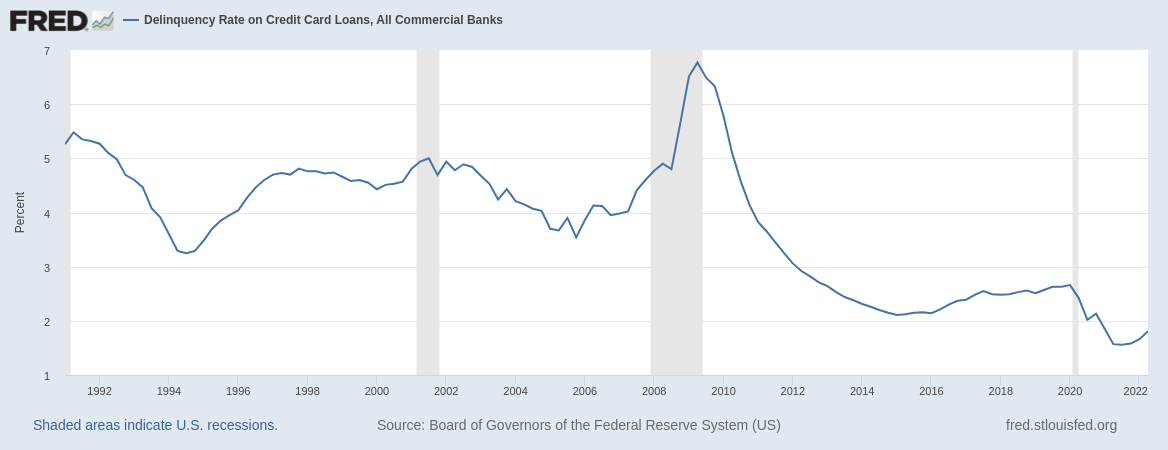
\includegraphics[width=1.0\textwidth]{fredgraph}
	\caption[Delinquency rate on credit card loans for the period 1992-2022]{Delinquency rate on credit card loans for the period 1992-2022{\citep{fedgraph_delinquency_history}}.}
	\label{fig:fredgraph}
\end{figure}

Existing models can be used to manage risk. However, developing models that perform better than those in use is feasible.

\subsection{Aim \& Approach}
The objective of this project was to explore different machine learning algorithms \& deep learning architectures on the American Express default prediction dataset\citep{amex-default-prediction-dataset} to predict if a customer will default on the payment in the future. The project work started by developing a model using classic machine learning algorithm \acf{SVM} followed by creating multiple models using Random Forest Classifier \& \acf{GBDT} algorithms. \acf{ANN}, \acf{GRU} \& Custom ensemble model created by model combining \acs{ANN}, \acs{GRU} and \acs{GBDT} were created as part of exploring deep learning architectures. Finally created a lean model, using less features \& optimzed parameters using \acs{GBDT} which provided comparable performances to the previously explored models.

\subsection{Structure of Report}
The remainder of the report is structured as follows: in Section \ref{sec:background_knowledge} background information on different machine learning \& deep learning algorithms along with metrics explanation is provided. Then in Section \ref{sec:literature_review} a literature review related to the credit card default prediction research is given. Section \ref{sec:materials} \& \ref{sec:methodology} provides detailed explanations on the dataset, tools \& software used in the project, and methodology followed for creating the models. Model evaluation results and the comparison is given in Section \ref{sec:results_discussions}. Finally Section \ref{sec:conclusion} discusses the conclusion of the project. 

\section{Background Knowledge} \label{sec:background_knowledge}
This section provides the reader with the required background information on the machine learning algorithms, deep learning architectures, data preprocessing techniques \& model evaluation metrics. The explanations provided in this section are at intutive level only without going deeper into the mathematical formulation.
\subsection{\acf{SVM}}
\acs{SVM} is a reliable classification and regression machine learning algorithm that maximizes the accuracy of a model without overfitting the training data. There are 4 main components to the \acs{SVM} model, Hyperplane, Support Vectors, Margin, Kernel function. Hyperplane refers to the decision boundary of the model, this could be a line if the data is 2 dimensional, plane if the data is 3 dimensional, or hyperplane if the data is n dimensional. Support Vectors refers to the data points that are nearest to the hyperplane and  these points are more difficult to classify. As shown in figure \ref{fig:svm}, the \acs{SVM} algorithm tries to find a hyperplane which maximizes the distance between the support vectors and the hyperplance and hence reducing the overfitting on the training set.
\begin{figure}[ht]
	\centering
	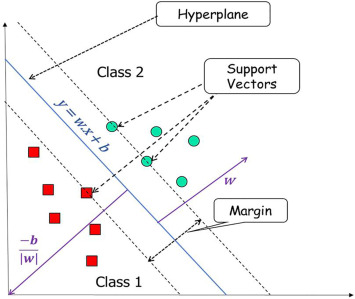
\includegraphics[width=0.4\textwidth]{svm}
	\caption[Support Vector Machine]{Components of \acs{SVM} \citep{rani2022machine}}
	\label{fig:svm}
\end{figure}
\acs{SVM} machinel learning technique uses a concept of Soft Margin to remove the issues that may arise due to outliers in the dataset.Additionally, if the decision boundary is non-linearly separable, \acs{SVM} transforms original data to map into new space using the Kernel function. Linear Kernel, Polynomial kernel \& \acf{RBF} are different kernel functions that can be used in \acs{SVM} model. There are multiple implementations of the \acs{SVM} technique is available; however, in this project libsvm\citep{chang2011libsvm} \& liblinear \citep{fan2008liblinear} is used as these implementations provide higher performance on large datasets.
\subsection{Ensemble Learning}
Ensemble methods are highly effective compared to the traditional machine learning techniques and considered state-of-the-art approach for solving many challenges \citep{sagi2018ensemble}. The idea behind ensemble learning technique is to train multiple base learners/models and combine the predictions from each learner to make the final prediction. As shown in figure \ref{fig:ensemble_learning}, ensemble techniques can be mainly categorized into 2 types Homogeneous \& Heterogeneous methods. In homogeneous methods all the base learners uses the same machine learning technique; on the other hand, heterogeneous methods may use different types machine learning techniques as the base learner.
\begin{figure}[ht]
	\centering
	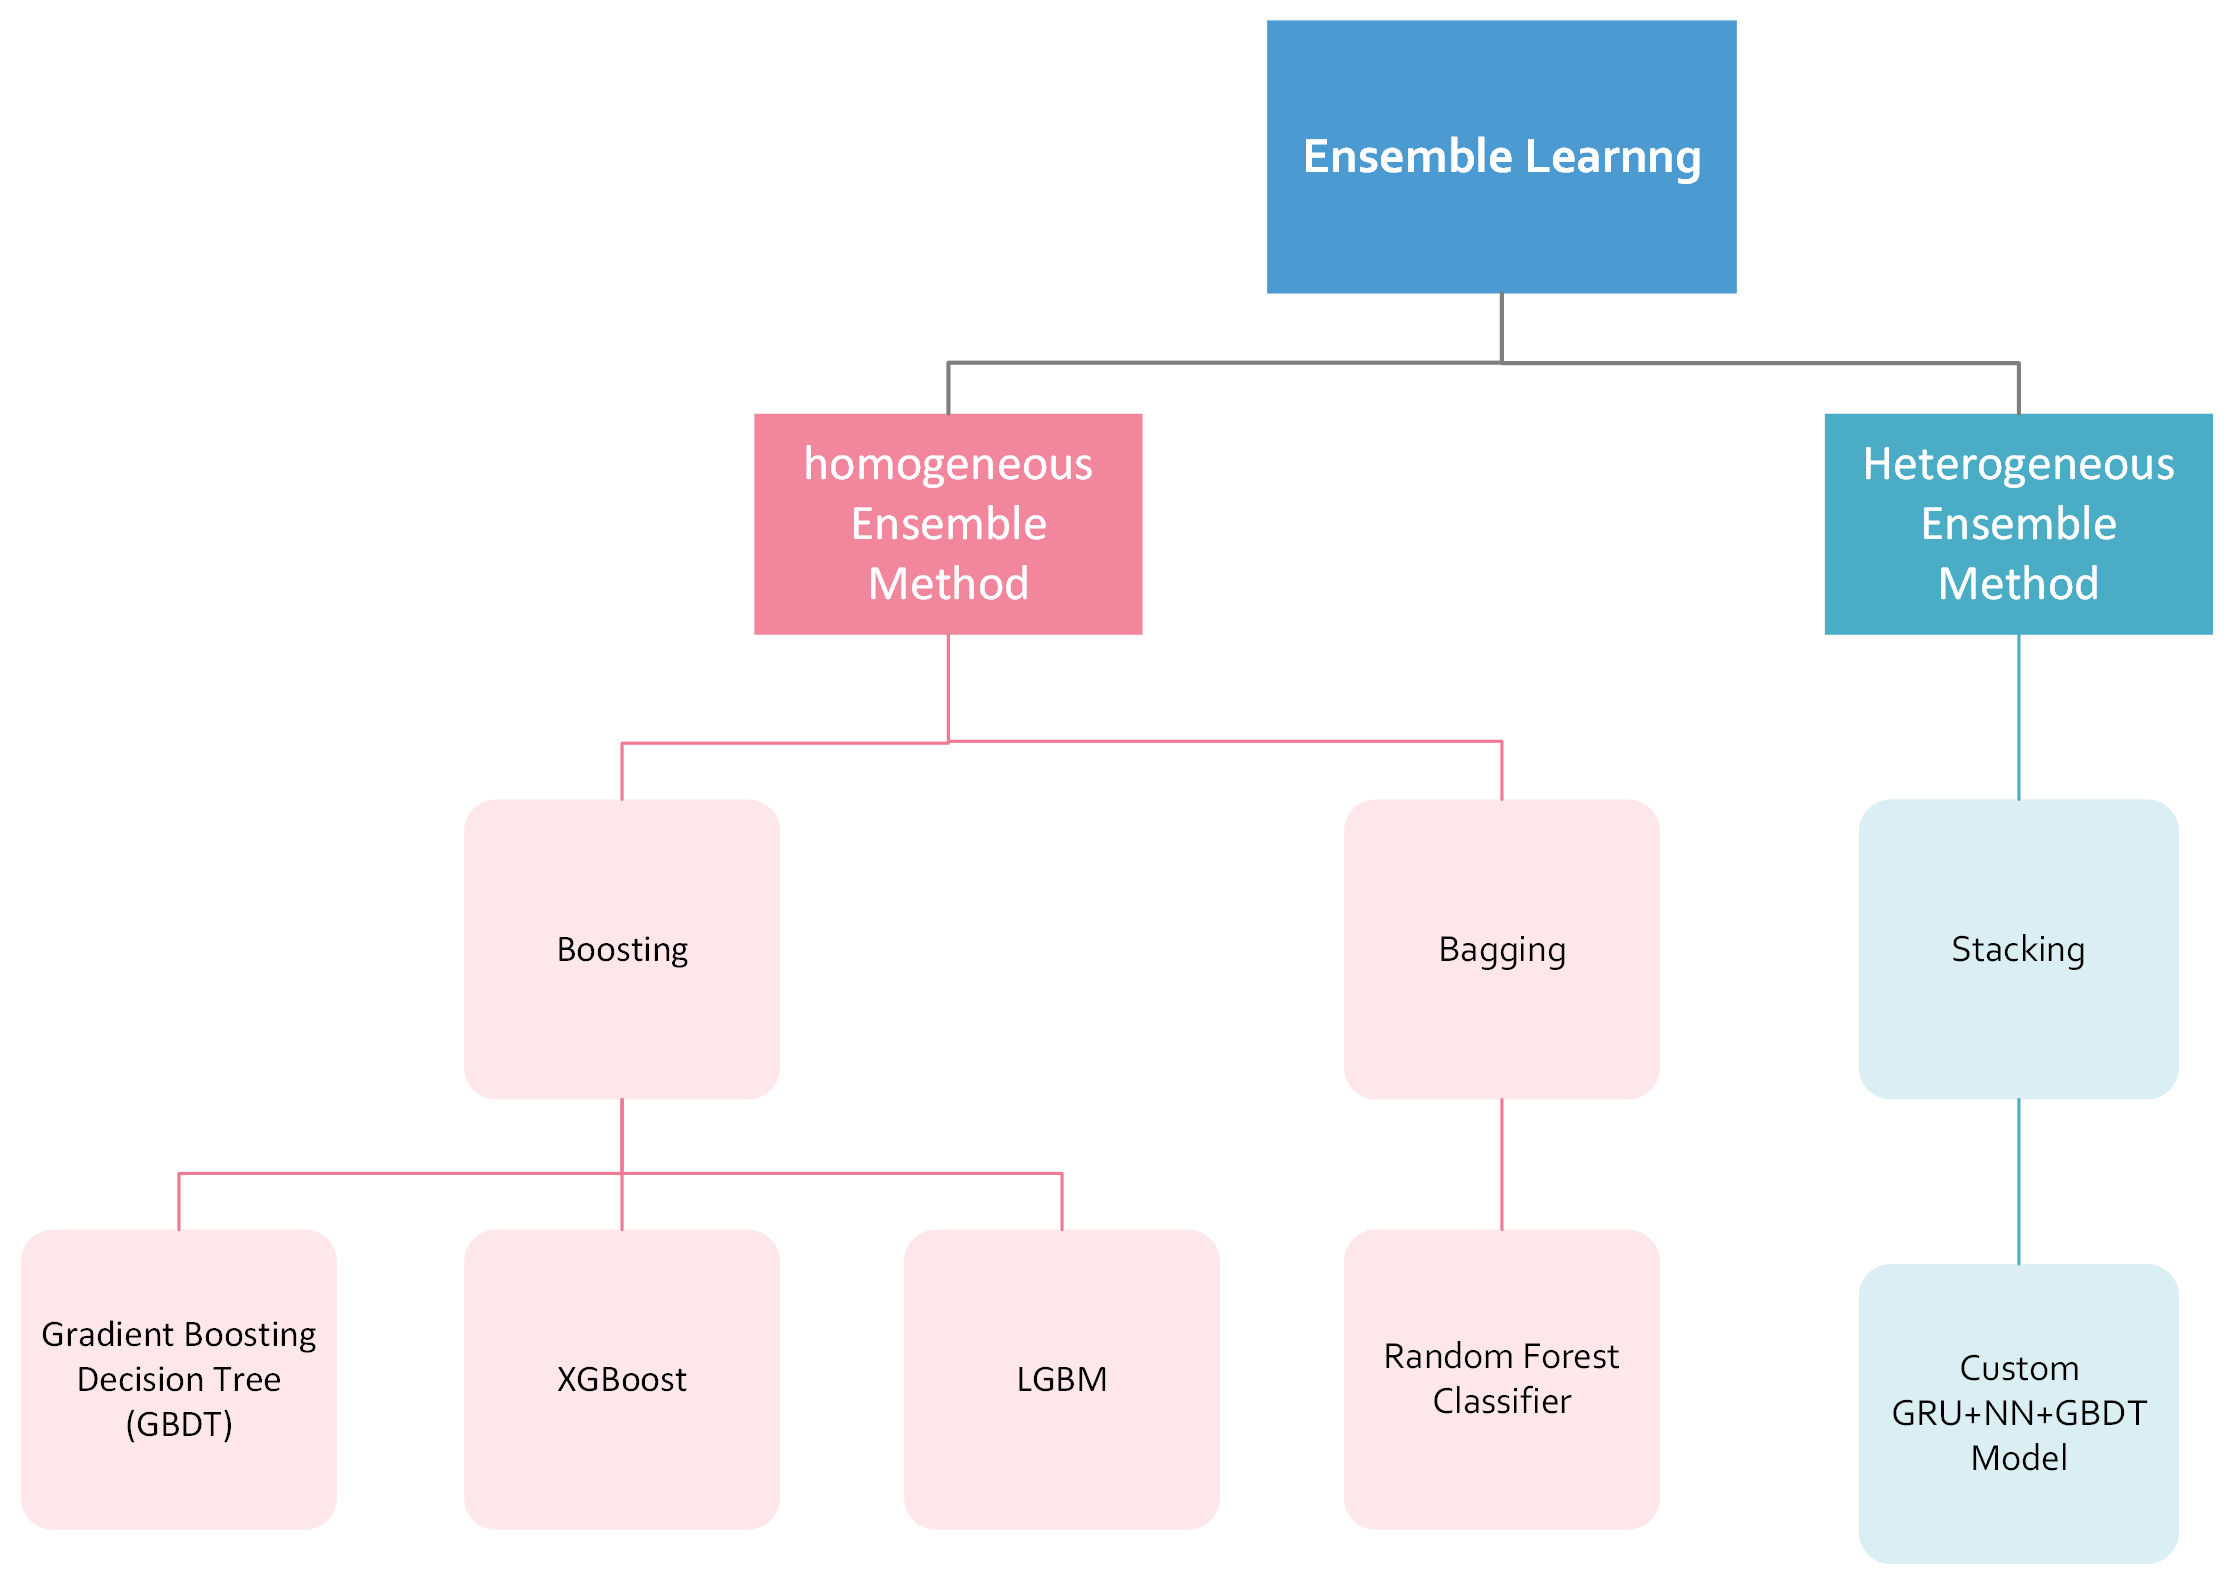
\includegraphics[width=0.5\textwidth]{ensemble_learning}
	\caption[Ensemble Learning Techniques]{Ensemble Learning Techniques \& Implementations}
	\label{fig:ensemble_learning}
\end{figure}
\subsubsection{Bagging}
Bagging is a Homogeneous Ensemble Method where the base learners are trained in parallel on the complete training set or a subset of training set based on the configuration. As depicted in figure \ref{fig:bagging_boosting}, initially creates multiple dataset through random sampling with replacement, then train the mutiple learners in parallel. Finally combine output from all learners using either taking average or using majority vote strategy based on the problem is being solved. 
\begin{figure}[ht]
	\centering
	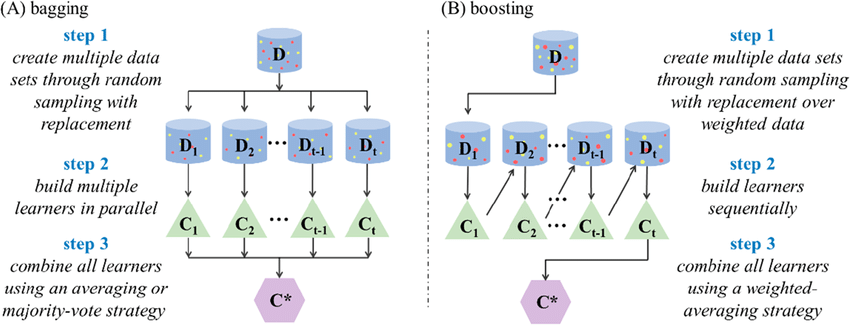
\includegraphics[width=0.5\textwidth]{bagging_boosting}
	\caption[Illustrations of bagging and boosting ensemble algorithms.]{Illustrations of bagging and boosting ensemble algorithms\citep{yang2019concepts}.}
	\label{fig:bagging_boosting}
\end{figure}
\subsubsection{Boosting}
Boosting is a Homogeneous Ensemble Method where the base learners are trained sequentially and the predictions from individual learners are combined to make the final prediction. The model starts by creating a base learner which performs slightly better than the random prediction, then subsequent learners try to improve on the prediction made by the previous learner. The process ends when the improvement made by the new learner is less than the threshold. As depicted in figure \ref{fig:bagging_boosting}, the boosting methods uses a weighted averaging strategy to combine the predictions from the individual learners. 
\subsubsection{Stacking}
Stacking is a Heterogeneous Ensemble Method where the output from the base learners is passed through another learner to make the final prediction. In Bagging \& Boosting methods the final prediction was made using taking average, majority voting, or weighted average; however the Stacking models uses a learner to make the final prediction. Figure \ref{fig:stacking} shows a sample Ensemble Stacking Model. Model A, B, and C are base learners which are trained parallely. The output from Model A, B \& C is then passed through a Generalizer/Meta Learner which predicts the final output. 
\begin{figure}[ht]
	\centering
	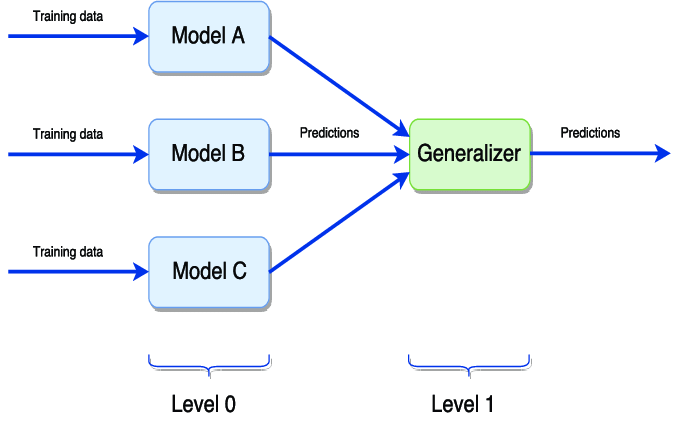
\includegraphics[width=0.5\textwidth]{stacking}
	\caption[An example scheme of stacking ensemble learning. ]{An example scheme of stacking ensemble learning \cite{divina2018stacking}.}
	\label{fig:stacking}
\end{figure}

\subsection{\acf{RF}}
\acf{RF} \citep{breiman2001random} is an ensemble bagging method technique which uses \acf{DT} to create base learners. \acs{DT} are a non-parametric supervised learning method used for classification and regression. The goal is to create a model that predicts the value of a target variable by learning simple decision rules inferred from the data features. \acs{RF} creates multiple \acs{DT} and trains each one of them with a random subsample of the dataset. The predictions from each \acs{DT} is then combined by either taking average or by using majority voting strategy.\\
\begin{figure}[ht]
	\centering
	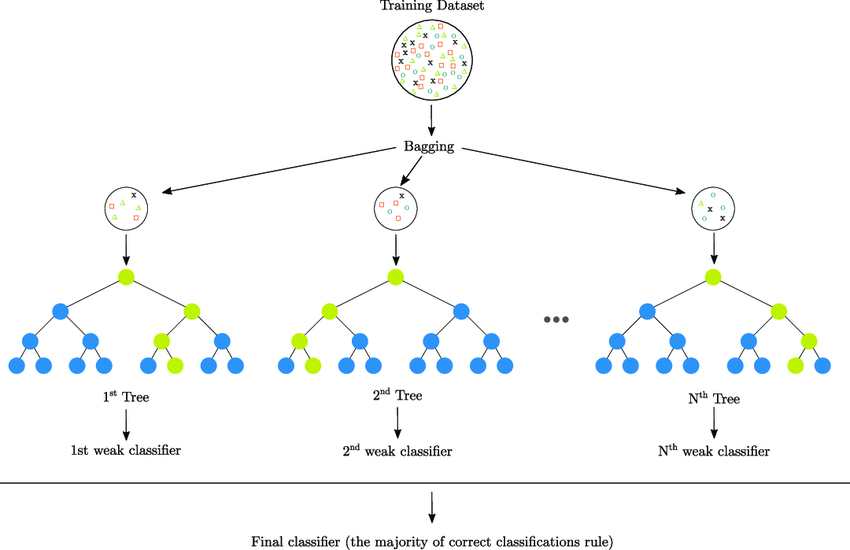
\includegraphics[width=0.5\textwidth]{random_forest}
	\caption[An example \acs{RF}. ]{An example of \acf{RF} \cite{sapountzoglou2020fault}.}
	\label{fig:random_forest}
\end{figure}

\subsection{\acf{GBDT}}
Gradient-boosted decision trees are a machine learning technique for optimizing the predictive value of a model through successive steps in the learning process. Each iteration of the decision tree involves adjusting the values of the coefficients, weights, or biases applied to each of the input variables being used to predict the target value, with the goal of minimizing the loss function (the measure of difference between the predicted and actual target values). The gradient is the incremental adjustment made in each step of the process; boosting is a method of accelerating the improvement in predictive accuracy to a sufficiently optimum value.
\begin{figure}[ht]
	\centering
	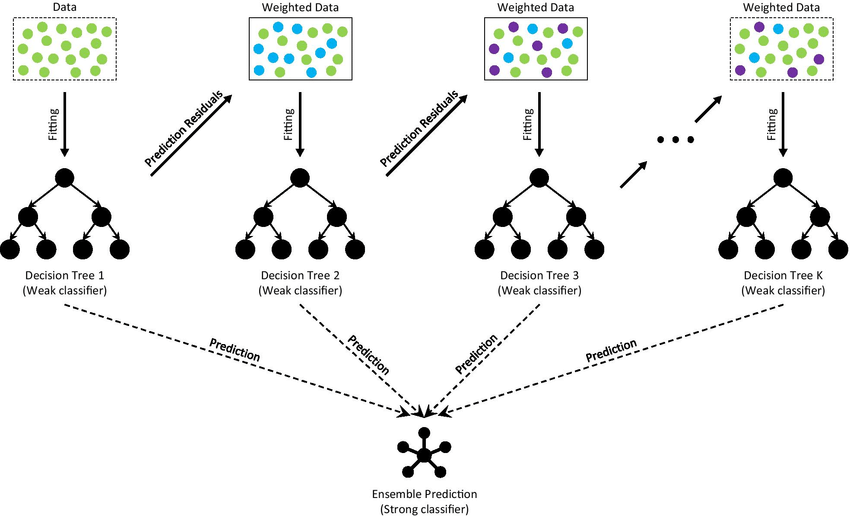
\includegraphics[width=0.5\textwidth]{gbdt}
	\caption[Architecture of \acf{GBDT}]{Architecture of \acf{GBDT} \cite{deng2021ensemble}.}
	\label{fig:gbdt}
\end{figure}
\subsubsection{\acf{XGBoost} \& \acf{LGBM}} \label{sec:xgboost_lgbm}
\acf{XGBoost}\citep{chen2016xgboost} and \acf{LGBM}\citep{ke2017lightgbm} are two mostly used \acf{GBDT} framework/libraries which performs much better than the basic \acs{GBDT} models \citep{machado2019lightgbm}. \acf{XGBoost} \& \acs{LGBM} frameworks differ in how the individual weak learners are constructed. As shown in figure \ref{fig:lgbm_xgboost_tree_growth}, the \acs{XGBoost} uses Level Wise Tree Growth strategy while the \acs{LGBM} uses Leaf Wise Growth Strategy. \acf{GOSS} technique is used by the \acs{LGBM} to split the nodes while generating the individual weak learners; on the other hand, the \acs{XGBoost} uses Pre-Sorted and historgram based algorithms for splitting nodes.

\begin{figure}[ht]
	\centering
	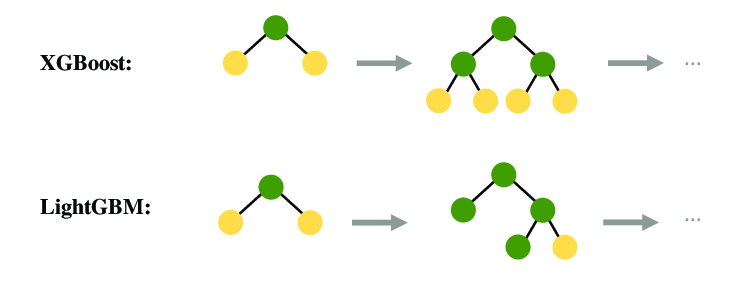
\includegraphics[width=0.5\textwidth]{lgbm_xgboost_tree_growth}
	\caption[\acs{XGBoost} Level wise tree growth and \acs{LGBM} Leaf wise tree growth.]{\acs{XGBoost} Level wise tree growth and \acs{LGBM} Leaf wise tree growth.\cite{rezazadeh2020generalized}.}
	\label{fig:lgbm_xgboost_tree_growth}
\end{figure}

Both frameworks require the features to be numerical and does not support text features; thus; categorical encoding must be done before training \acs{LGBM} \& \acs{XGBoost} models.
In addition, both these libraries are well optimized for parallel processing and hence can be used for large datasets.

\subsection{\acf{ANN}}
\acs{ANN} are a subset of Machine Learning algorithms. The  architecture and name of \acs{ANN} is inspired by how the human brains works, specifically, how biological neurons signal to one another\citep{ibm2022neural}. Figure \ref{fig:ann} represents the architecture of a \acs{ANN} in general. The network consists of an input layer, multiple hidden layers and an output layer. There are multiple nodes, also known as neurons, in each layer. The neurons are the building blocks of the \acs{ANN} network. Each neuron connects to all the neurons in the next layer; moreover, neurons in the input layer are basically the input features.

\begin{figure}[ht]
	\centering
	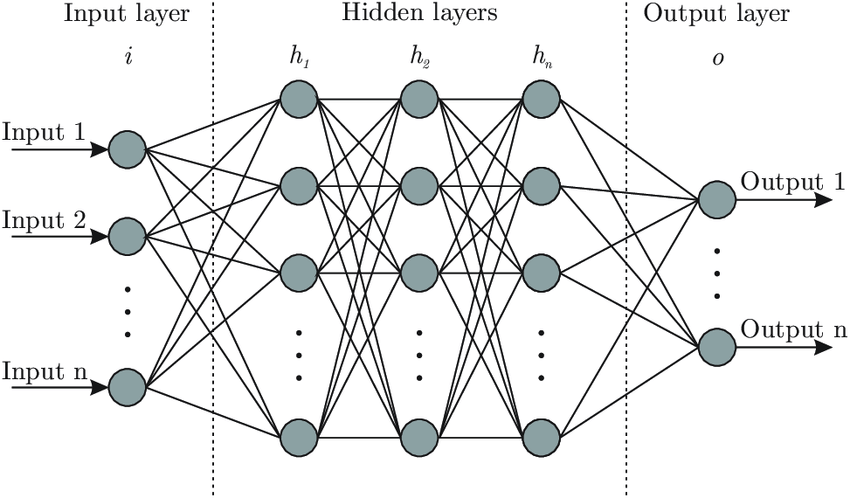
\includegraphics[width=0.5\textwidth]{ann}
	\caption[Architecture of \acf{ANN}.]{Architecture of \acf{ANN}\cite{bre2018prediction}.}
	\label{fig:ann}
\end{figure}
Neurons are the basic building block of an \acs{ANN}. As shown in figure \ref{ann_node}, each neuron at least consists of a learning function and an activation function. Learning function can be thought of as a simple logistic/linear regression model and the activation function can be though of as a gatekeeper which decides how much influence this neuron should have in the next layer. Commonly used activation functions are Sigmoid, \acs{ReLU} and tanh. 
\begin{figure}[ht]
	\centering
	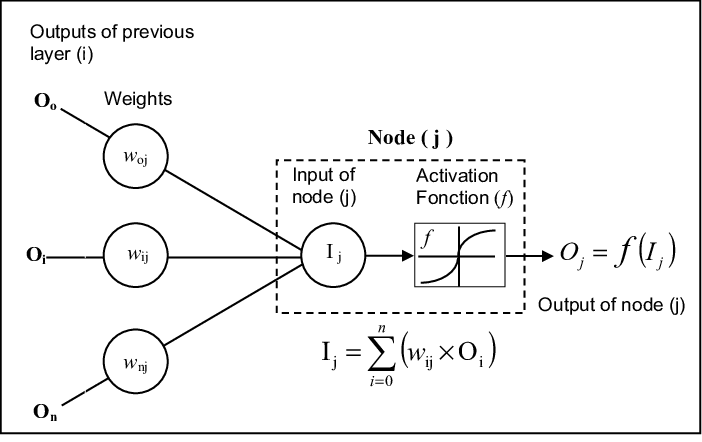
\includegraphics[width=0.5\textwidth]{ann_node}
	\caption[Representation of a Neuron in \acf{ANN}.]{Representation of a Neuron in \acf{ANN}.\cite{ghedira2004effect}}
	\label{fig:ann_node}
\end{figure}

While training \acs{ANN} models, a cost function is assigned to evaluate the performance of the model, \acf{MSE}, Binary Cross Entropy are some of the cost functions which are generally used. Finally the weights learning function of each neuron is adjusted through an algorithm called Backpropogation based on the result of the cost function. The algorithm ends when the cost function converges (figure \ref{fig:cost_function}) and the improvement made to the performance is less than the threshold.
\begin{figure}[ht]
	\centering
	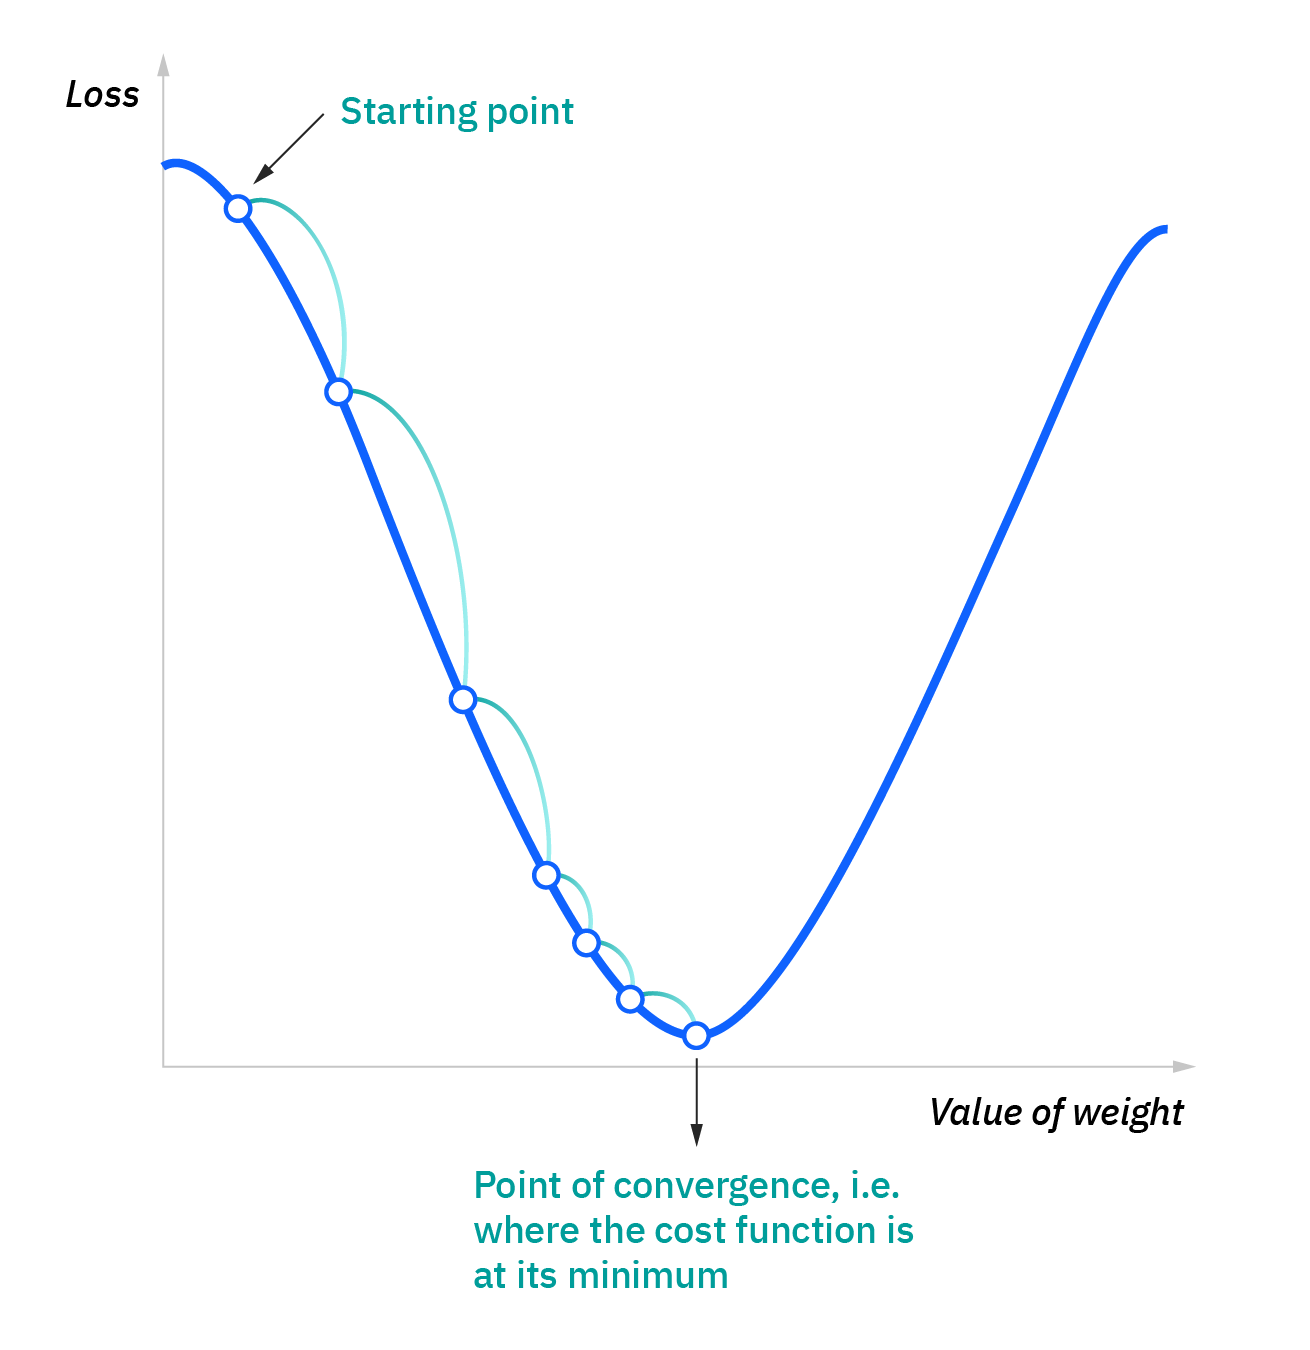
\includegraphics[width=0.5\textwidth]{cost_function}
	\caption[Representation of Convergence of Cost Functions]{Representation of Convergence of Cost Functions\citep{ibm2022neural}}
	\label{fig:cost_function}
\end{figure}

\subsection{\acf{RNN}}
A \acf{RNN} is a type of \acs{ANN} which uses sequential data or time series data. \acs{RNN} has the capability of using previous inputs in the sequence to influence the current input and output, in other words, the \acs{RNN} has a memory of past events/data which it uses to calculate the current output.Figure \ref{fig:rnn_nn} shows comparison of a normal feed forward neural network (Tradition Neural Network)  and a \acs{RNN}. In a Feed Forward Neural Network the signals flow only in one direction from input to output; however, In an \acs{RNN} output of a layer is added to the next input and fed back into the same layer.Traditional Deep Learning networks assumes no dependency between the inputs and outputs, on the other hand, the output of \acs{RNN} depends on the previous inputs in the sequence.
\begin{figure}[ht]
	\centering
	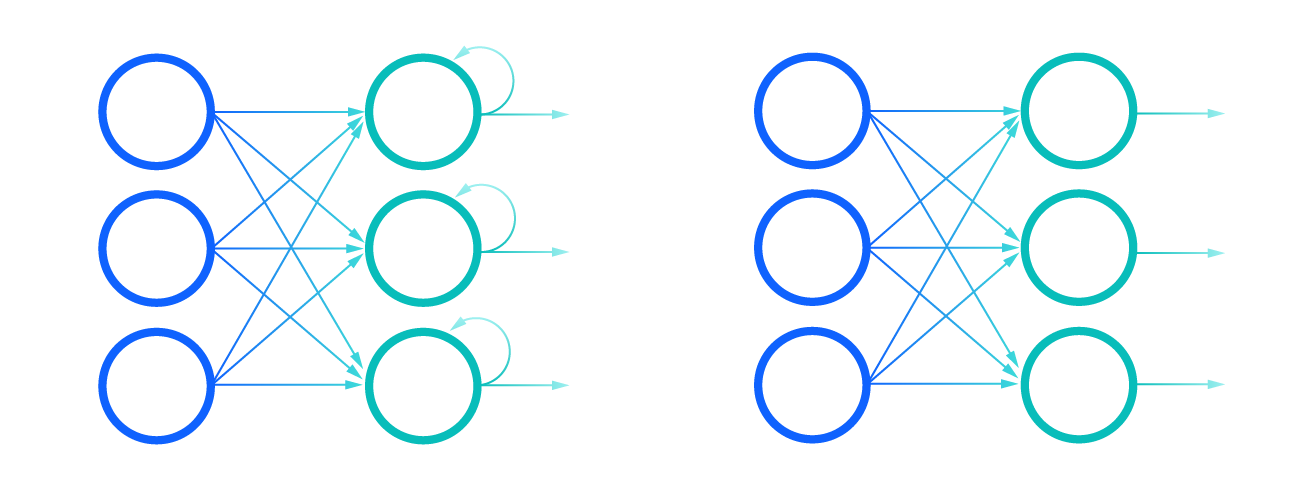
\includegraphics[width=0.5\textwidth]{rnn_nn}
	\caption[Comparison of Recurrent Neural Networks (on the left) and Feedforward Neural Networks (on the right)]{Comparison of Recurrent Neural Networks (on the left) and Feedforward Neural Networks (on the right)\citep{ibm2022rnn}.}
	\label{fig:rnn_nn}
\end{figure}

Consider the Credit Card Default problem with 12 month data, the Rolled \acs{RNN} represents the entire Neural Network, and the Unrolled \acs{RNN} represents each layer in the Neural Network or each time step. In credit card default problem, X\textsubscript{0}  represents the data for the first month, X\textsubscript{1} for the second month and so on. \acs{RNN} uses \acf{BPTT} algorithm and gradient descent to learn the weights of the model while training.
\begin{figure}[ht]
	\centering
	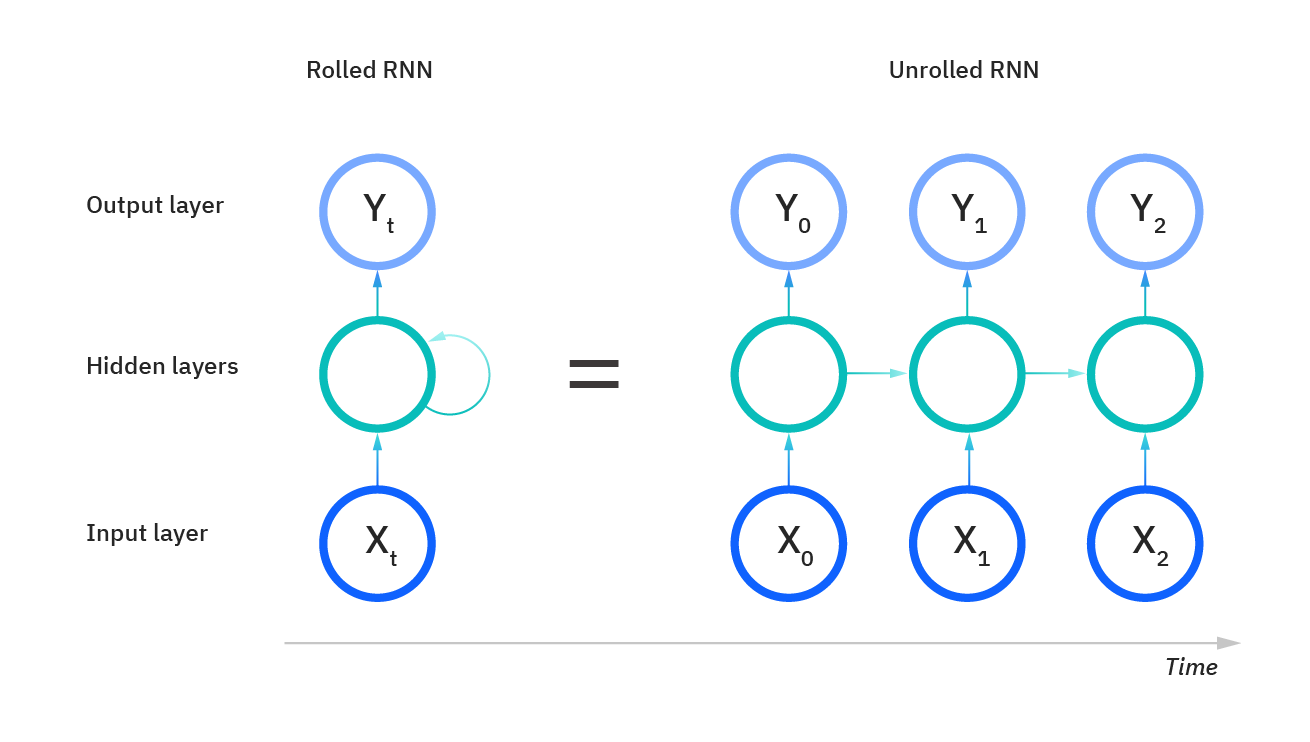
\includegraphics[width=0.5\textwidth]{rnn_rolled_unrolled}
	\caption[\acs{RNN} rolled and unrolled]{\acs{RNN} rolled and unrolled \citep{ibm2022rnn}.}
	\label{fig:rnn_rolled_unrolled}
\end{figure}


There are 3 variants of the \acs{RNN} architectures as shown in figure \ref{fig:various_rnn}. While \acs{RNN} uses previous inputs to influence the current output, \acs{BRNN} use future inputs as well to improve the accuracy of the \acs{RNN} architecture. \acf{LSTM} is variant of \acs{RNN} proposed Sepp Hochreiter and Juergen Schmidhuber in their paper \citep{hochreiter1997long}. If the previous input which is influencing the current input is not in recent past, \acs{RNN} might not be able predict the current output accurately. \acs{LSTM} tries to solve this issue using cells in the hidden layers of the neural network. Cells have three different gates, input, output and forget gate, these gates control the flow of information which is needed to predict the output in the network. \acf{GRU} is similar to \acs{LSTM} and tries to resolve the issue of Short-term memory issue of \acs{RNN}. \acs{GRU} uses hidden states to regulate the information in the network and uses two gates, reset, update gate, to control the flow of information through network \citep{cho2014learning}.\\
\begin{figure}[ht]
	\centering
	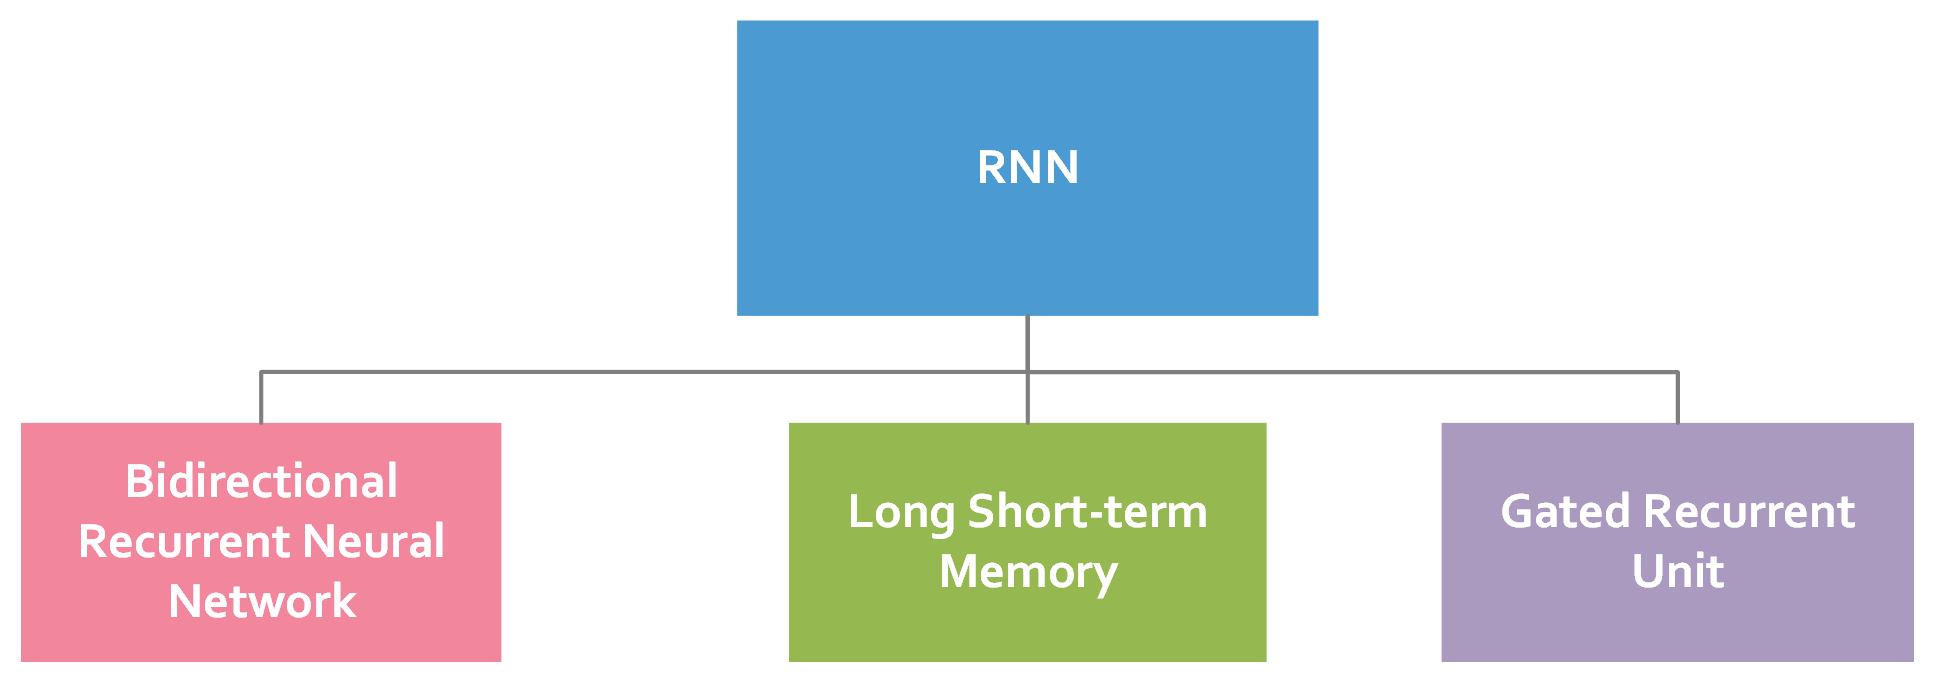
\includegraphics[width=0.7\textwidth]{various_rnn}
	\caption[Variant \acs{RNN} Architectures]{Variant \acs{RNN} Architectures.}
	\label{fig:various_rnn}
\end{figure}

\subsection{\acf{GRU}}

\acf{GRU} is a variant of \acs{RNN} network which tries to solve the short-term memory issue of \acs{RNN} networks. Figure \ref{fig:gru_new} represents the structure for \acs{GRU} unit. Input to the current unit is the output hidden state from the previous input (h\textsubscript{t-1});furthermore, \acs{GRU} has two gates, update(z\textsubscript{t}) and reset(r\textsubscript{t}) gate. The algorithm uses reset gate to calculate the candidate output state (h\textsubscript{t}\textsuperscript{'}). Finally, update gate z\textsubscript{t}, previous hidden state h\textsubscript{t-1} and candidate output hidden state h\textsubscript{t}\textsuperscript{'} are used to calculate the final output hidden state h\textsubscript{t}.
\begin{figure}[ht]
	\centering
	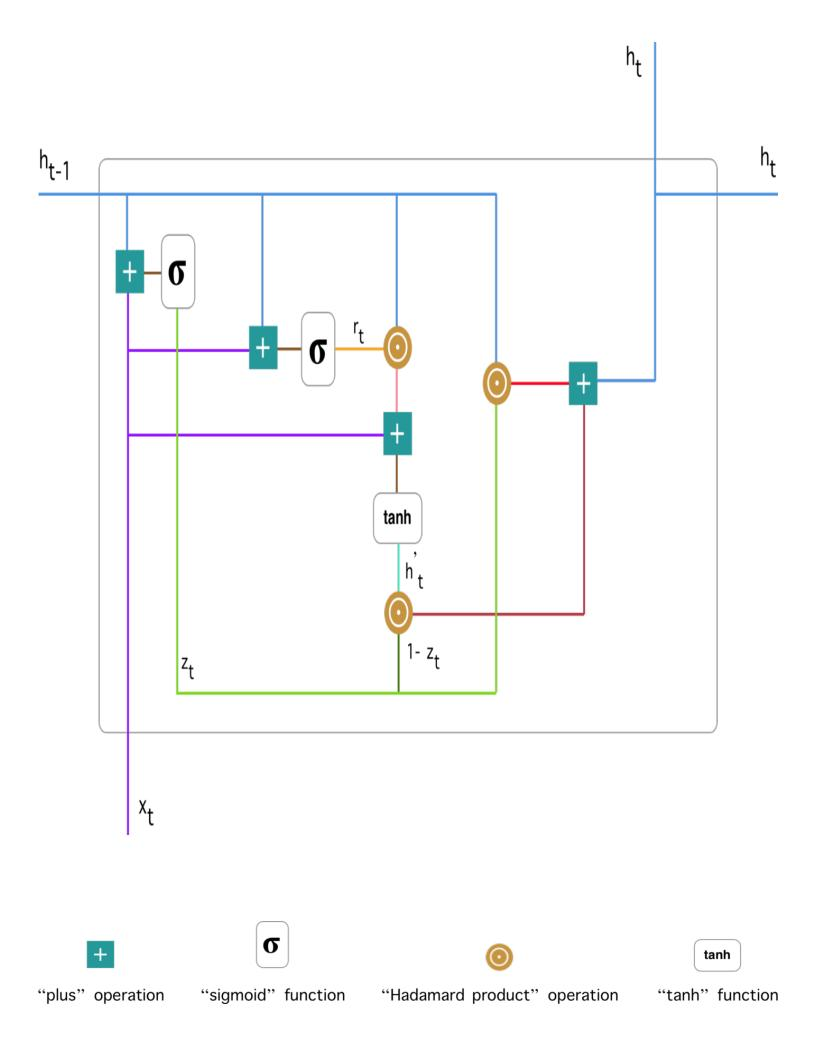
\includegraphics[width=0.7\textwidth]{gru_new}
	\caption[\acs{GRU} Architecture]{\acs{GRU} Architecture}
	\label{fig:gru_new}
\end{figure}

Update gate is calculated using equation \ref{eq:gru_ugate} which is highlighted in figure \ref{fig:gru_detail} (a) of update gate. Update gate is formed adding the result of multiplication of  input x\textsubscript{t} with its own weight W\textsuperscript{z} and previous hidden state , h\textsubscript{t-1} with it's own weight U\textsuperscript{z}. Finally applying Sigmoid activation function to make the value between 0 and 1. Update gate determines how much of the information from the previous time steps needs to be passed to the future.
\begin{equation} \label{eq:gru_ugate}
	\centering
	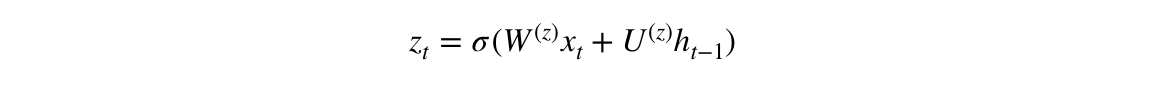
\includegraphics[width=0.7\textwidth]{gru_ugate_eq}	
\end{equation}

Reset gate is calculated using equation \ref{eq:gru_rgate} which is highlighted in figure \ref{fig:gru_detail} (b). Reset gate may seem similar to update gate by looking at the formula;;however, the important thing to note is that the weights are different for update \& reset gate and hence it learns different characteristics of the network. Reset gate determines how much of the memory from past inputs to forget.

\begin{equation} \label{eq:gru_rgate}
	\centering
	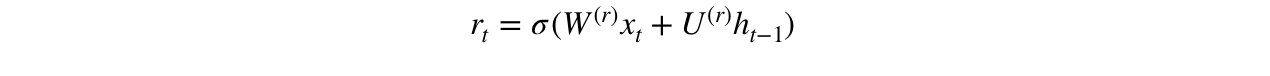
\includegraphics[width=0.7\textwidth]{gru_reset_eq}	
\end{equation}

Calculation of new candidate output hidden state is shown in equation \ref{eq:gru_cstate_} and \ref{fig:gru_detail} (c). Both the input and previous output hidden state is multiplied by the respective weights before taking sum. Additionally, the product of previous hidden state and the weight is further multiplied (Hadamard Product) with the reset gate, this operation determines how much of the previous information to be passed over to the current output hidden state.
\begin{equation} \label{eq:gru_cstate}
	\centering
	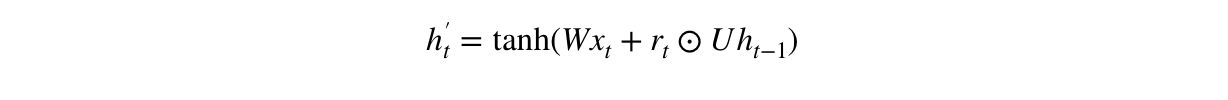
\includegraphics[width=0.7\textwidth]{gru_cstate_eq}	
\end{equation}

Finally the update gate, previous output hidden state and the candidate current output hidden state is used to calculate the final current output state as shown in equation \ref{eq:gru_nstate} and figure\ref{fig:gru_detail} (d). 
\begin{equation} \label{eq:gru_nstate}
	\centering
	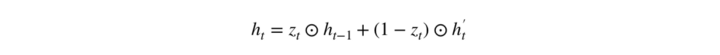
\includegraphics[width=0.7\textwidth]{gru_nstate_eq}	
\end{equation}

\begin{figure}[h!]
	
	\begin{subfigure}{0.49 \textwidth}
		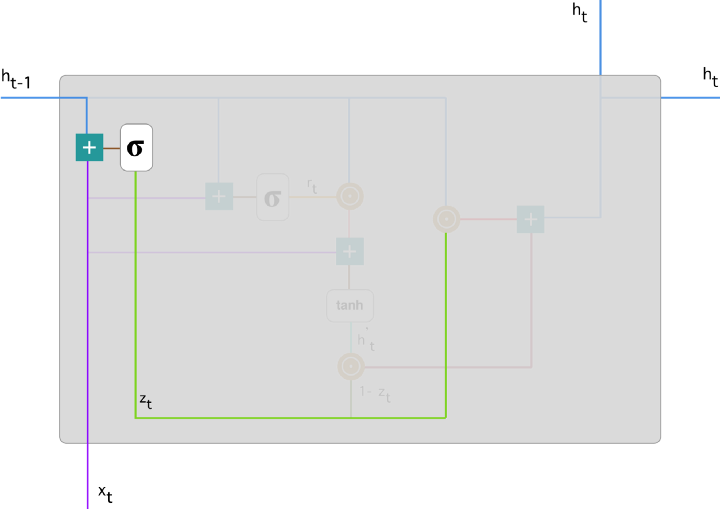
\includegraphics[width=1\linewidth, height=1\linewidth]{gru_ugate}
		\subcaption[Update Gate]{Update Gate}
		\label{fig:gru_ugate}
	\end{subfigure}
	\hfill
	\begin{subfigure}{0.49 \textwidth}
		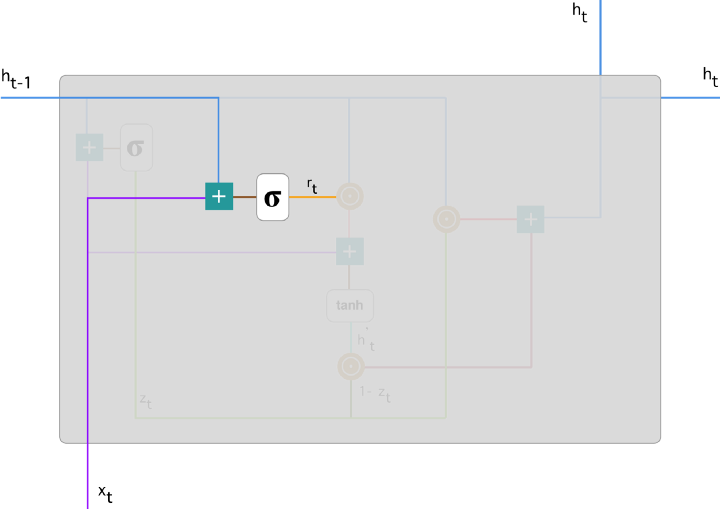
\includegraphics[width=1\linewidth, height=1\linewidth]{gru_rgate}
		\caption[Reset Gate]{Reset Gate}
		\label{fig:gru_rgate}
	\end{subfigure}
	\begin{subfigure}{0.49 \textwidth}
		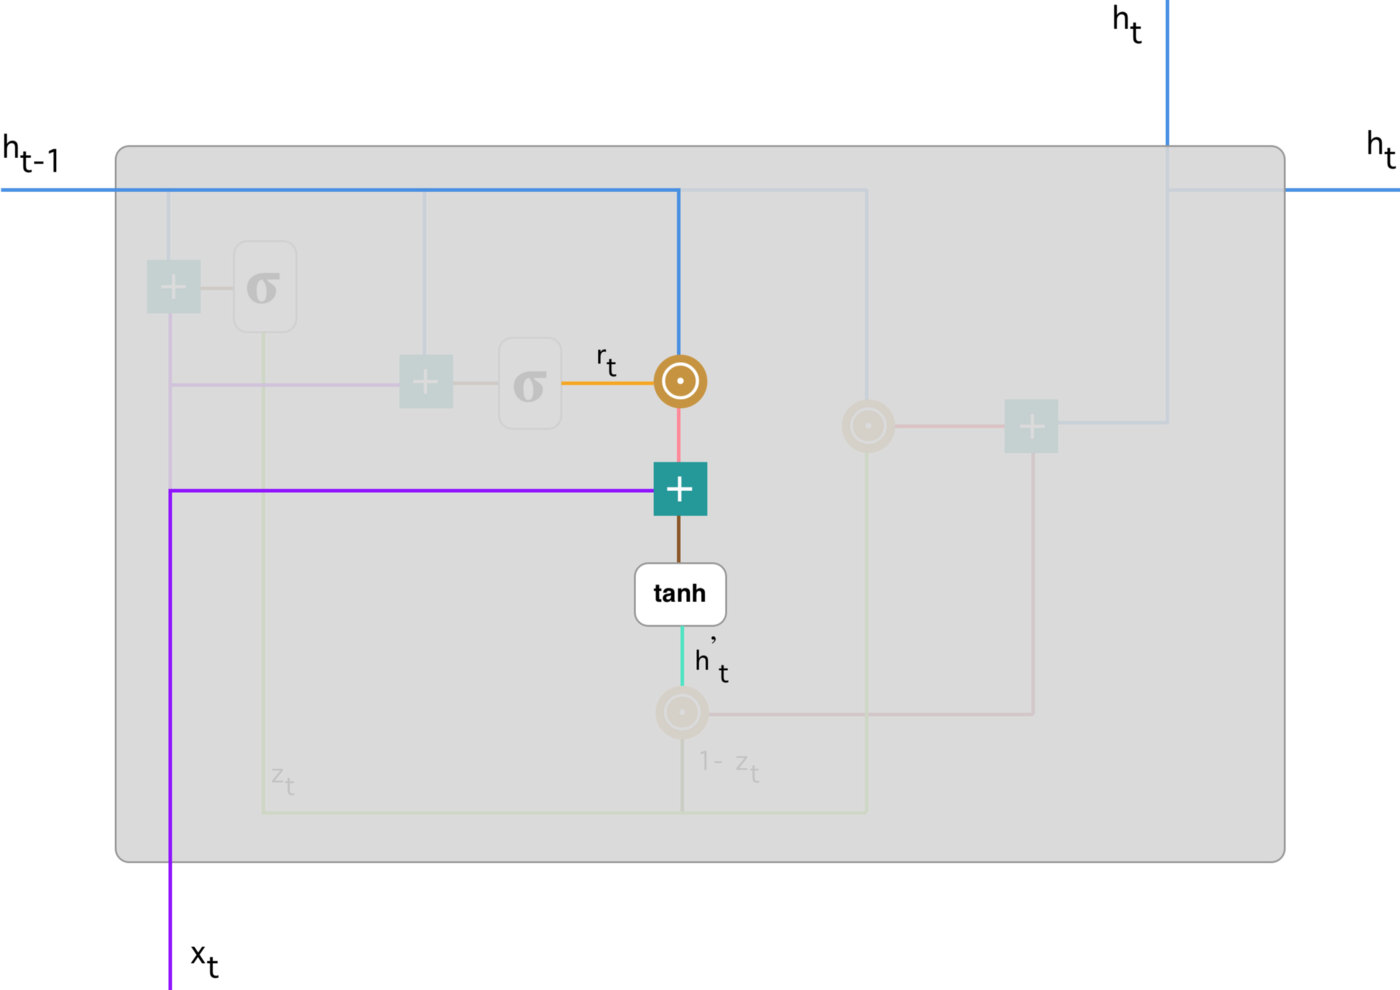
\includegraphics[width=1\linewidth, height=1\linewidth]{gru_cstate}
		\caption[Candidate Output State]{Candiate Output State}
		\label{fig:gru_cstate}
	\end{subfigure}
	\hfill
	\begin{subfigure}{0.49 \textwidth}
		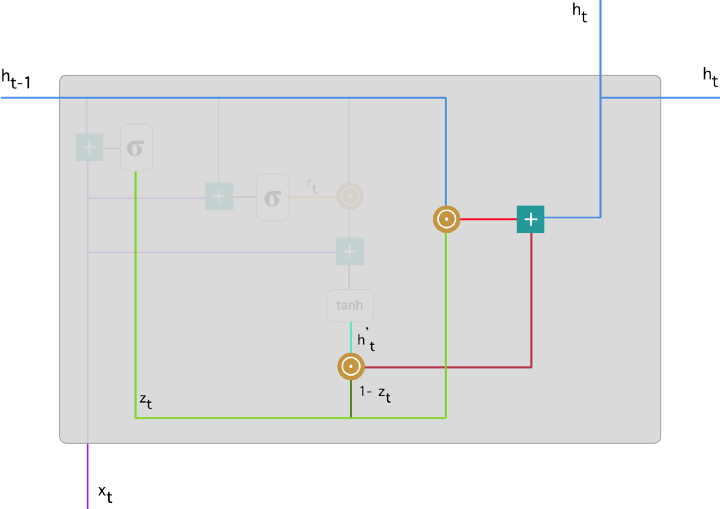
\includegraphics[width=1\linewidth, height=1\linewidth]{gru_nstate}
		\caption[Final Output State]{Final Output State}
		\label{fig:gru_nstate}
	\end{subfigure}
	\caption[\acs{GRU} Architecture Stepwise]{\acs{GRU} Architecture Stepwise \citep{simeon2017gru}}
	\label{fig:gru_detail}
\end{figure}

\subsection{Feature Selection}
While building a Machine Learning model, all of the features might not contribute equivalently to the model's prediction performance, some of the features might impact the model's prediction performance adversely. This problem becomes more prominent on high dimensional data. The process of identifying the important features which improve the performance of the model is called Feature Selection. Two feature selection methods which were used in this project are Select From Model \& Sequential Feature Selection.
\subsubsection{Select From Model}
In this method, the training dataset is first trained on a machine learning model which is computationally less expensive and provides acceptable level of performance, this model can be considered as a filter. Then remove the features whose feature weights are less than the threshold value in the filter model. Finally, use the filtered dataset for training the main model. In this project, the \acs{SVM} is used as the filter model for training the main \acs{LGBM} model.
\subsubsection{Sequential Feature Selection}
As shown in figure \ref{fig:seq_feature_selection}, sequential feature selection starts with a subset of dataset and then an estimator chooses the best feature to add or remove to the dataset based on the \acf{CV} score obtained by adding/removing each feature. The process ends once the algorithm reaches the exit criteria. Exit criteria could be either the count of features or until improvement in performance gained by adding/removing features is not greater than a threshold.
\begin{figure}[ht]
	\centering
	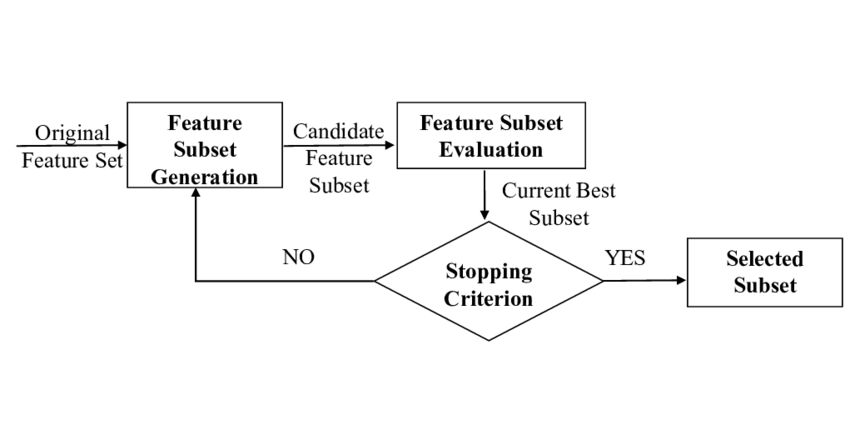
\includegraphics[width=0.5\textwidth]{seq_feature_selection}
	\caption[Sequential Feature Selection Flowchart]{Sequential Feature Selection Process\citep{beyan2015detection}}
	\label{fig:seq_feature_selection}
\end{figure}
There are two types Sequential Feature Selection techniques, Forward Selection \& Backward Selection. In Forward Selection, the initial feature subset contains only one feature, then additional features are added based on \acs{CV} score until the exit criteria is met. On the other hand, in Backward Selection technique, the initial feature subset contains all the features, then the algorithm removes the features based on \acs{CV} score until the exit criteria is met. 
\subsection{Encoding Categorical Features}
As discussed in section \ref{sec:xgboost_lgbm}, some of the machine learning techniques does not support categorical text variables. Two most common methods used to encode categorical features are Ordinal Encoder \& One-hot encoder. Ordinal encoder is better than the One-hot encoder in memory efficiency.
\subsubsection{Ordinal Encoder}
In this method, the feature is transformed into a numerical value by assigning numbers to each distinct category. For eg: in Scikit Learn library the categorical variables low, medium, high will be transformed to 0, 1, 2; moreover, a default number can be assigned to categories which are not seen in the training dataset. 
\subsubsection{One-hot Encoder}
In this method, the categorical feature column is transformed into n different features each representing one distinct category. For eg: a feature X with low,medium,high as distinctive categorical values, will be transformed into 3 features X\_low, X\_medium, X\_high. X\_low will have a value of 1 if the X='low' for the record, likewise for the other features.
\subsection{Data Oversampling}
A classification data set with skewed class proportions is called imbalanced. Classes that make up a large proportion of the data set are called majority classes. Those that make up a smaller proportion are minority classes. Data sampling is a method used to overcome / reduce the effect of Class Imbalance on the performance of the model. There two types of Data Sampling, Over Sampling \& Under Sampling. Over Sampling techniques boost the minority class entries by introducing new records in minority class; on the other hand, the Under Sampling methods eliminates entries from majority class and makes the majority \& minority class entries to similar proportion.

In this project, Data Oversampling techniques are used as the dataset is large. \acf{SMOTE} \citep{chawla2002smote} \&  KMeans \acs{SMOTE} \citep{last2017oversampling} are two different Oversampling methods which were explored in this project.

\subsubsection{\acf{SMOTE}}
\acs{SMOTE} method introduces new data points in the minority class by finding nearest neighbors and adding new data point along the line of nearest neighbor. Figure \ref{fig:smote} shows the \acs{SMOTE} process, in this picture green points are minority class \&  blue points are majority class. The algorithm first selects a data point from the minority class, then finds the K nearest neighbors among the minority class. Finally one of the K nearest neighbor is choosen randomly and a new synthetic minority class data point (red) is added along the straight line connecting the selected data point and the choosen nearest neighbor.

\begin{figure}[ht]
	\centering
	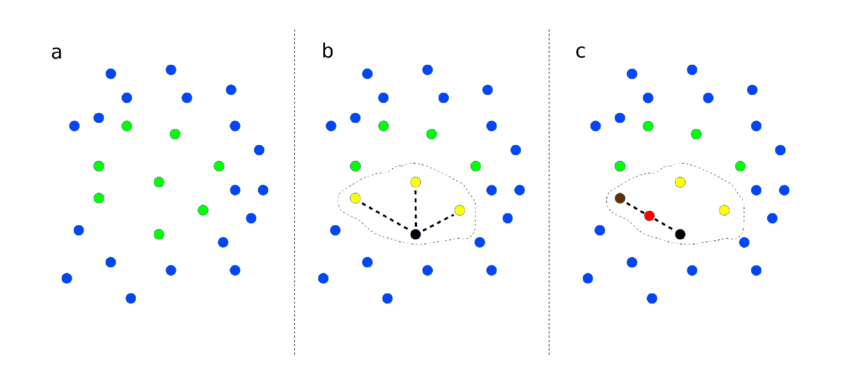
\includegraphics[width=0.5\textwidth]{smote}
	\caption[\acs{SMOTE} algorithm]{\acs{SMOTE} algorithm \citep{schubachimbalance}}
	\label{fig:smote}
\end{figure}
\subsubsection{KMeans \acs{SMOTE}}
In KMeans \acs{SMOTE} method, the minority class is first passed through a KMeans clustering model before applying the \acs{SMOTE} algorithm. Clustering before applying \acs{SMOTE} helps to eliminate the problem of oversampling the outliers in the minority classes;moreover, clustering also helps to apply the \acs{SMOTE} algorithm for non-linearly separable data. As shown in  figure \ref{fig:kmeans_smote}, the SMOTE algorith is applied separately on each cluster.
\begin{figure}[ht]
	\centering
	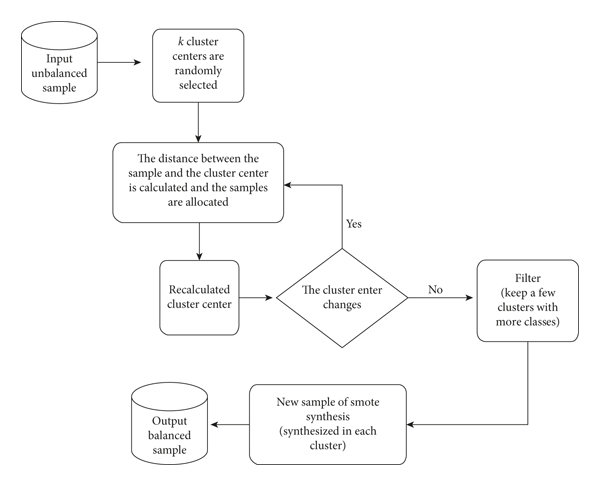
\includegraphics[width=0.5\textwidth]{kmeans_smote}
	\caption[KMeans \acs{SMOTE} algorithm]{KMeans \acs{SMOTE} Flowchart \citep{chen2021research}}
	\label{fig:kmeans_smote}
\end{figure}

\subsection{Metrics}
Figure \ref{fig:confusion_matrix} represents the Confusion Matrix associated with classification problem. There are 4 important terms related to confusion matrix, \acf{TP}, \acf{TN}, \acf{FP}, and \acf{FN}. \acs{TP} represents the predictions where the truth label and the predicted labels are both positive; on the other hand, \acs{FP} represents the predictions where the predicted label is predicted label is positive but the truth label is negative. \acs{TN} represents the predictions where both the predicted label and the truth label are Negative. Predictions where the predicted label is negative and the truth label is positive is called \acs{FN}.
\begin{figure}[ht]
	\centering
	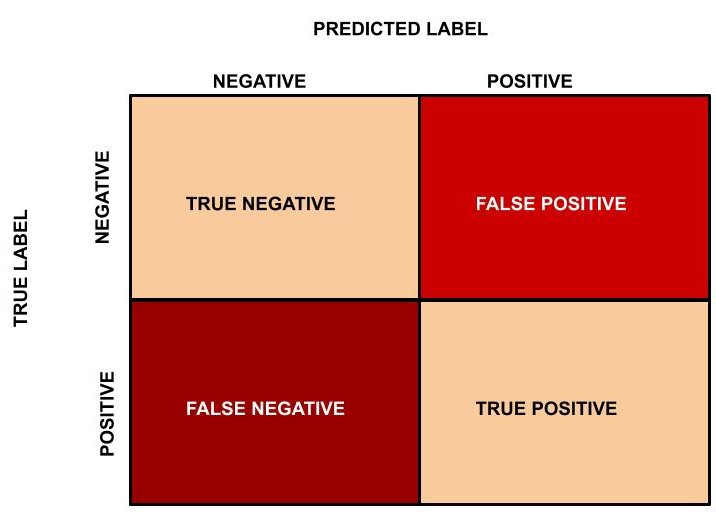
\includegraphics[width=0.5\textwidth]{confusion_matrix}
	\caption[Confusion Matrix]{Confusion Matrix \citep{confusion_matrix}}
	\label{fig:confusion_matrix}
\end{figure}
There are multiple metrics based on the confusion matrix, metrics which are relevant to this project is discussed in below sections.
\subsubsection{Accuracy}
Accuracy is defined as the ratio of total number of correct predictions and total number of samples. However, the Accuracy metric might be misleading on imbalanced dataset;for example, in a dataset where the minority class is only one percent of the overall dataset, 99\% can be achieved by predicting every data point as majority class. Equation \ref{eq:accuracy} shows the formula for calculating Accuracy.
\begin{equation} \label{eq:accuracy}
	Accuracy = \frac{TP+TN}{TP+TN+FP+FN}
\end{equation}
\subsubsection{Recall}
Recall represents the ratio of total number of positive predictions and the total number of positive samples. Intuitively, Recall provides an idea of how many positive samples where correctly identified by the model;for example, in a credit card default prediction dataset, recall is how many of the defaulted customers were identified by the model. Equation \ref{eq:recall} shows the formula for calculating Recall.
\begin{equation}\label{eq:recall}
	Recall = \frac{TP}{TP+FN}
\end{equation}
\subsubsection{Precision}
Precision is defined as the ratio of correct positive predictions and the total number of positive predictions. Precision provides insight into how many of the predicted positive samples where actually correct.Equation \label{eq:precision} shows the formula for calculating Precision.
\begin{equation}\label{eq:precision}
	Precision = \frac{TP}{TP+FP}
\end{equation}

\subsubsection{F1-Score}
F1-Score combines both Precision \& Recall into a single metric;in other words, F1-Score is the harmonic mean of Precision and Recall metrics. F1-Score has shown to be a good metric on the imbalanced datasets classification problems. F1-Score better represents the performance of the model on the dataset compared to the other metrics. Equation \ref{eq:f1score} shows the formula for calculating the F1-Score.
\begin{equation}\label{eq:f1score}
	Precision = 2 * \frac{Precision*Recall}{Precision + Recall}
\end{equation}
\subsection{\acf{CV}}
\subsubsection{K-Fold \acs{CV}}
\subsection{Hyper Parameter Tuning}
\subsubsection{Grid Search CV}
\subsection{Stochastic Gradient Descent}
\subsection{File Format}
\subsubsection{Parquet}
\subsection{Binary Cross Entropy}
\subsection{Summary}

\section{Literature Review}\label{sec:literature_review}
\subsection{Introduction}
This section discusses the current techniques used to predict the credit card default. Since the dataset used for these studies differ, a direct comparison of results is not possible. However, an overall comparison of different techniques and its efficiency in predicting the credit card default will be discussed wherever possible.

\subsection{Previous Work}
\citep{sayjadah2018credit} developed logistic regression, rpart decision tree \& Random Forest Classifier models on dataset generated from credit card operations. The dataset contains 30000 records and 24 features. A \acf{CFS} technique was used to reduce the dimensionality of the dataset. 30\% of the dataset was used as the test set for evaluating the performance. \citep{sayjadah2018credit} found that the Random Forest Classifier provided highest \acf{AUC} among the models.\\

\citep{widyadhanacredit} developed Logistic Regressiion, \acs{SVM}, \acs{ANN} \& Random Forest Classifier models to preduct credit card default on dataset containing 1000 records and 11 features. The dataset contains credit card data from cardholders from the territory of Indonesia;moreover, the authors used \acf{PCA} to do feature selection also. The dataset is split into 70:30 Train/Test set and the \acs{AUC} was used to compare the results. The authors found that the Random Forest Classifier outperformed all other models by far and provided a 80\% \acs{AUC} score.\\

\citep{hsu2019enhanced} approached the credit card default prediction from a different perspective and proposed a model where dynamic features (time dependent features) were first passed through a \acf{RNN} network to extract the time dependent features. Then the extracted dynamic features were concatenated with the static features and trained on a Random Forest Classifer. The dataset contained 30,000 samples credit card payment history with 23 features (5 static feature, 18 dynamic features). The authors compared the results of the proposed model with the \acs{SVM}, Logistic Regression and KNN models and found that proposed method outperformed the others and provided a \acs{AUC} score of 78\%.

\citep{alam2020investigation} investigated different approaches to solve the credit card default prediction problem with a specific focus on Class Imbalance. The credit card default prediction dataset are inherently imbalanced as only a small fraction of customers default on credit card. The authors employed different data under/over sampling techniques and evaluated performance on multiple credit card default dataset. They found that \acs{GBDT} classifier when used with KMeans \acs{SMOTE} provided the best results and the models performed significantly better on balanced datasets compared to imbalanced datasets.

\citep{faraj2021comparison} research shows that ensemble  methods  consistently  outperform  Neural  Networks  and  other  machine  learning algorithms in terms of F1 score. \citep{faraj2021comparison} uses the same dataset as the \citep{sayjadah2018credit} which has 30,000 records and 24 features. The authors found that \acs{XGBoost} provided maximum F1 score compared to Neural Networks, Random Forest Classifier and custom ensemble stacking model. Authors also concludes that the performance of \acs{XGBoost} model did not improve on balanced datasets. This observation was in contrary to the observations made by \citep{emil2019enhancing}, the authors of earlier had found that the best performance is achieved on \acs{GBDT} with KMeans \acs{SMOTE} method.

\subsection{Summary}
In conclusion, the ensemble boosting models generally provided better performance than the classic machine learning and deep learning techniques. The data under/over sampling had mixed performances depending on the dataset, some performed better with under/over sampling and some did not. Out of data under/over sampling techniques, KMeans \acs{SMOTE} performed better. Some studies used feature selection techniques in the data preprocessing techniques which improved the model efficiency. The studies discussed in the section used dataset which were imbalanced and  contained atmost 30,000 records; however, \citep{amex-default-prediction-dataset} contains 5 Million records and exploring the different techniques on such large scale dataset will help us to consolidate the understanding gained from these papers.


\section{Materials}\label{sec:materials}

\subsection{Primary Dataset}
The primary dataset contains 190 aggregated profile features of 458913 American Express customers at each statement date for 13 months. Features are anonymized and normalized, and fall into the following general categories:

\begin{itemize}
	\item D\_* = Delinquency variables
	\item S\_* = Spend variables
	\item P\_* = Payment variables
	\item B\_* = Balance variables
	\item R\_* = Risk variables	
\end{itemize}

This dataset\citep{amex-default-prediction-dataset} was released as part of the "American Express - Default Prediction" hosted in Kaggle by the American Express team.

\subsection{Secondary Dataset}
The secondary dataset was derived from primary dataset by applying the below mathematical aggregate operations to the numerical features.
\begin{itemize}
	\item Minimum 
	\item Maximum
	\item Mean
	\item Last Value
	\item Standard Deviation
\end{itemize}

Aggregate for the categorical features were taken by the applying below operations.
\begin{itemize}
	\item Last Value
	\item Count
	\item Unique Value Count
\end{itemize}

The secondary dataset contains 920 features and 458913 records.

\subsection{Tools \& Software}
The primary programming language used for the implementation of this project is Python version 3.7. Data analysis and manipulation is done using Pandas(1.3.5), seaborn(0.11.2) \& Dask(2.12.0) packages. Scikit Learn(1.0.2) package is used for create, train \& evaluate machine learning models. \acs{ANN} \& \acs{GRU} models were created using Tensorflow (2.8.2).Google colab was used to train the model in cloud and Github was used as the version control \& project management software.

\vfill
\clearpage
\section{Methodology}\label{sec:methodology}
\subsection{Introduction}
This section will first provide a brief overview of the overall strategy of the experiments performed as part of this project followed by  providing detailed explanation on the data preprocessing techniques used. Then in subsequent sections each experiment/model will be presented along with the model specific explanations \& details.

\subsection{Overview of Methodology Followed}
Figure \ref{fig:methodology} represents a overview of methodology in general followed for conducting experiments. The dataset was first split into chunks and stored in different files in parquet format to optimize the memory usage. Then, dataset was preprocessed to remove invalid values and encode categorical text variables to numerical values. Followed by data pre-processing, the dataset was split into Training \& Test set, this ensures that none of the entries in test set will have an influence in model training and model selection process. Then the dataset was enhanced using oversampling techniques to resolve the class imbalance issue;in addition, feature selection techniques were used to eliminate the features from the dataset which were less important and hence contribute very little to model. 
\begin{figure}[ht]
	\centering
	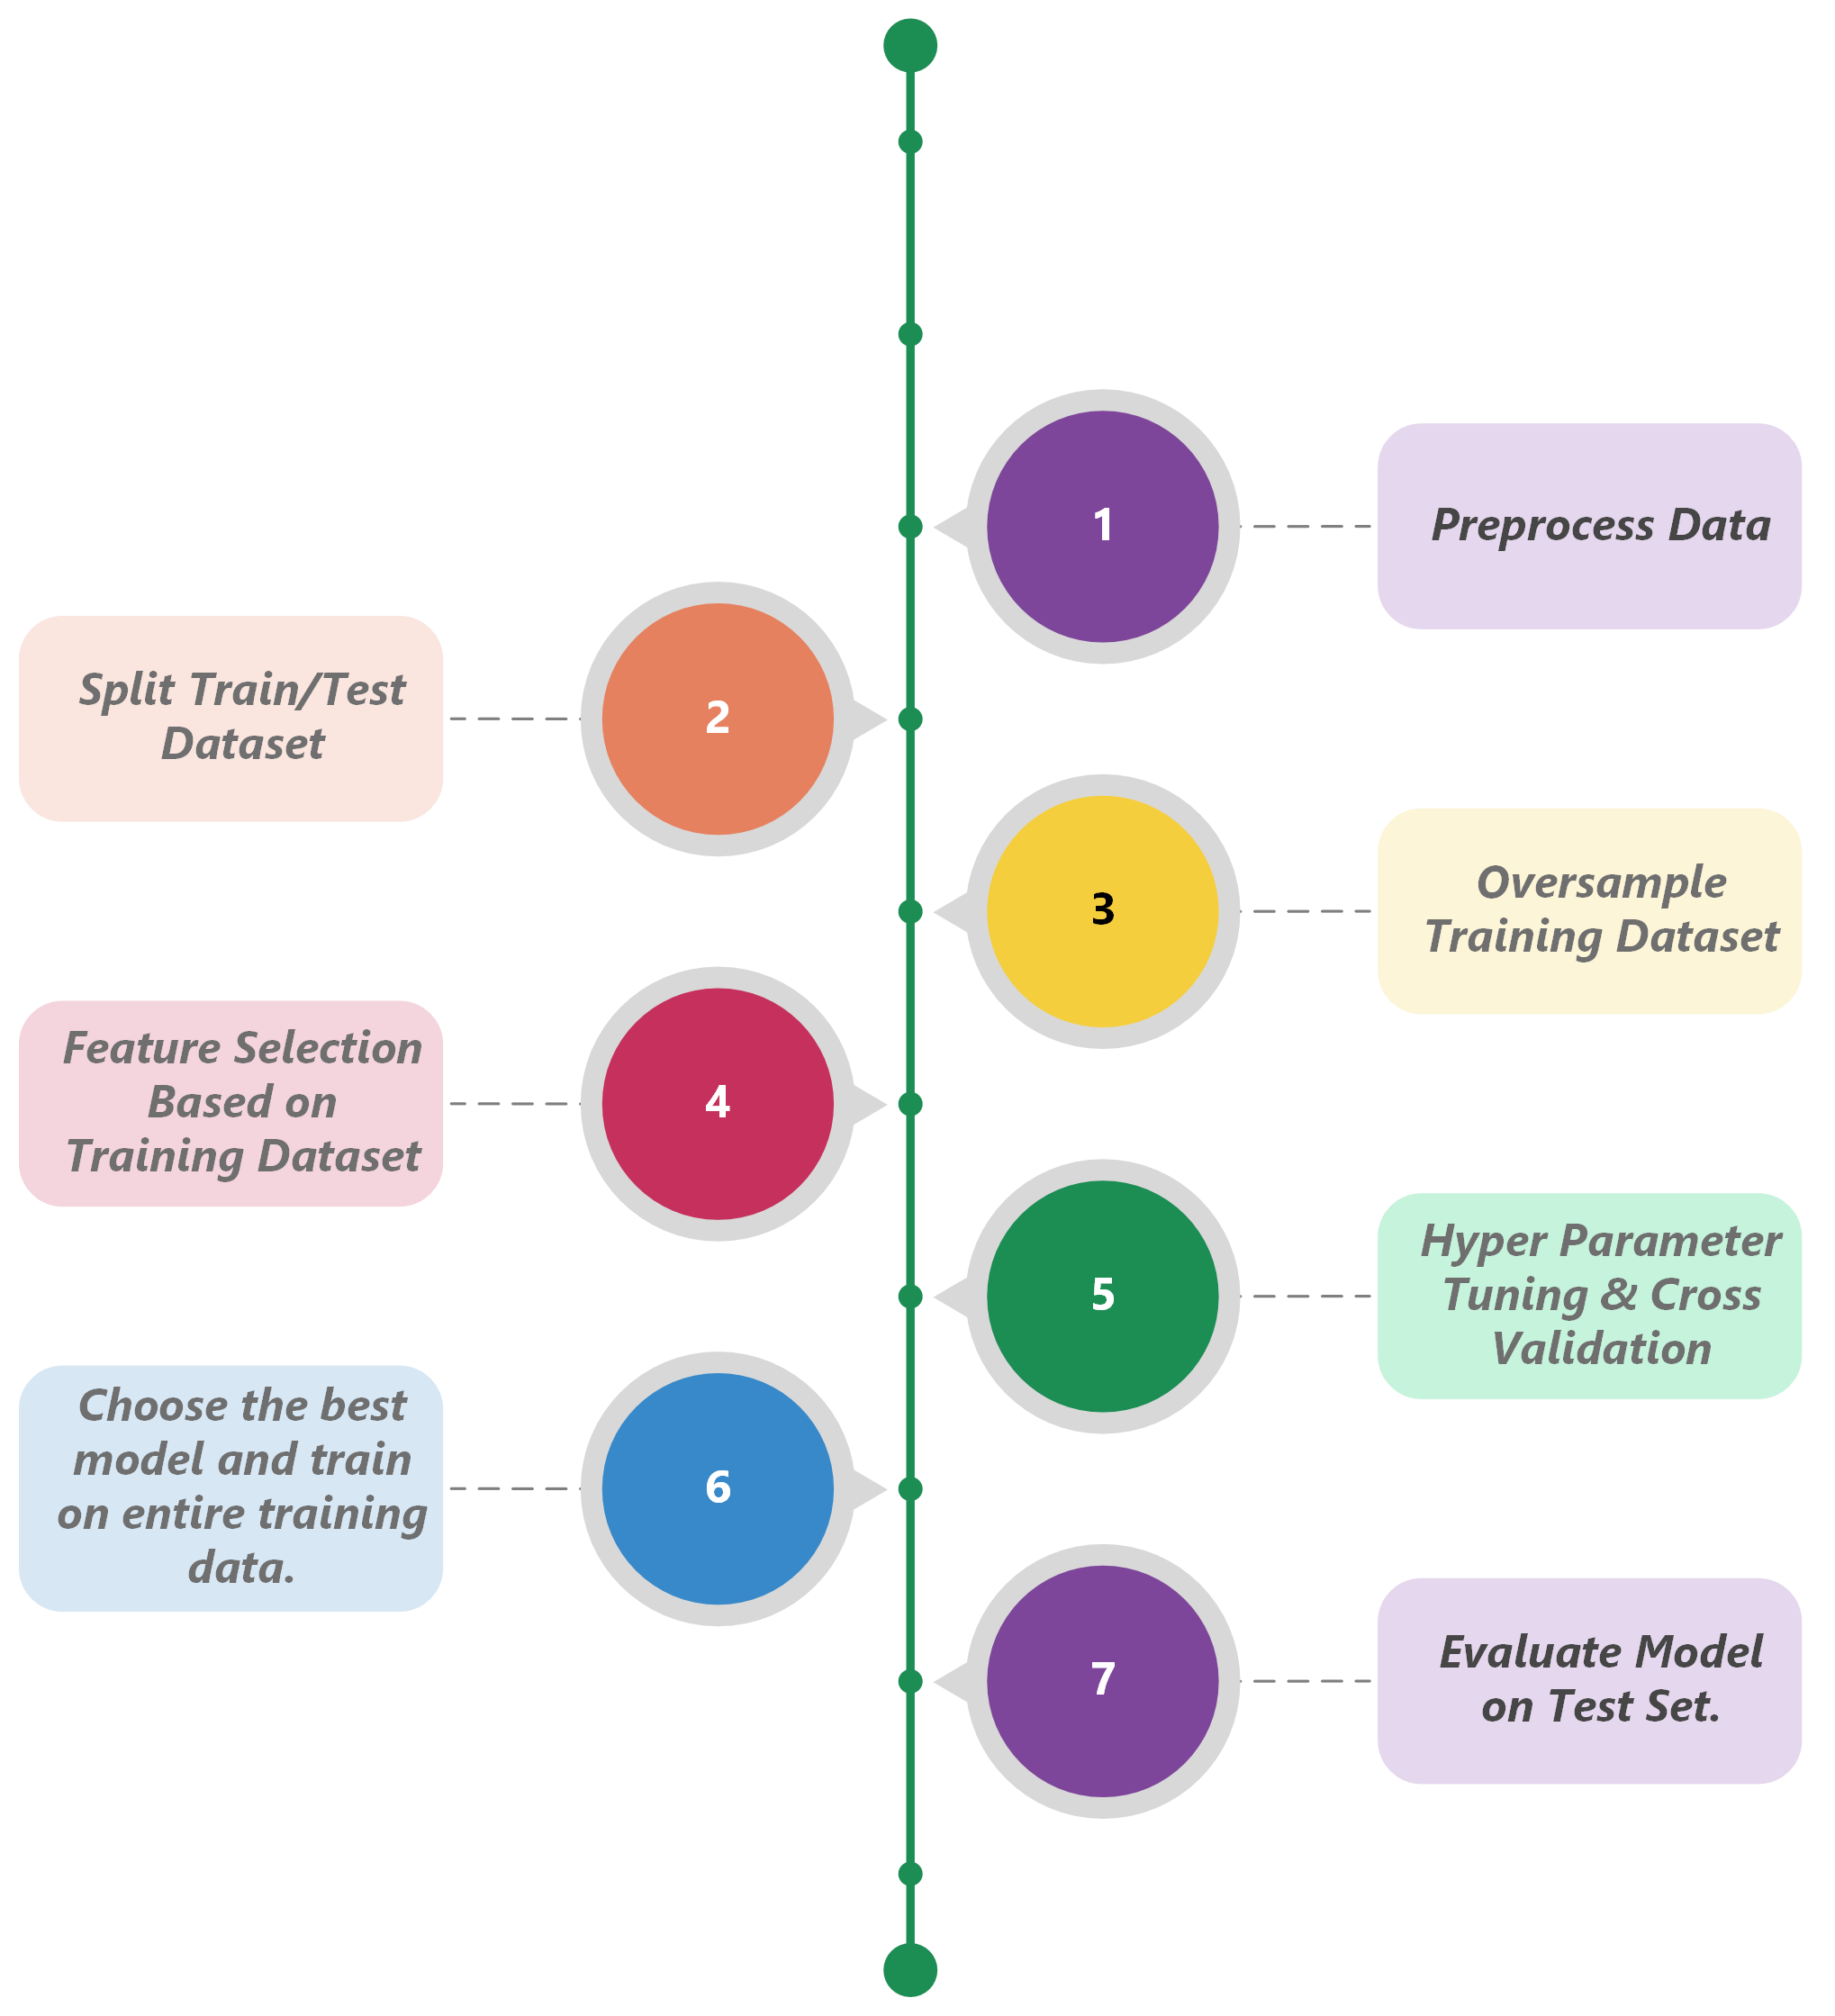
\includegraphics[width=0.8\textwidth, height=0.5\textheight]{methodology}
	\caption[Methodology]{Methodology followed for the experiments}
	\label{fig:methodology}
\end{figure}

After the feature selection, the model was created and then passed through a Hyperparameter tuning pipeline which helps to find the best parameters for the model which would give highest cross validation score. Finally the entire training dataset was trained on the best model found using hyperparameter tuning and the model was evaluated using the test set set aside at the beginning of the experiment.

\subsection{Data Preprocessing} 
This section discusses the common preprocessing techniques used in all experiments conducted as part of the project. The model specific data preporcessing techniques used will be discussed in respective sections describing the model.

\subsubsection{Default Values}
NaN \& NULL values in the dataset was replaced by Zero and if a column contains all values same, it was removed from the dataset. -1 was used as the default value for the categorical variables. The categorical variables were encoded using Ordinal Encoder before passing to the model training pipeline.

\subsubsection{Normalization}
The primary dataset from American Express is already normalized and all the values lies between zero to ten, hence none of the data normalization techniques were used to preporcess the data.
\subsubsection{Handling Memory Issue}
Google Colab provides 24 GB of \acf{RAM} in the  virtual environment, though the Primary Dataset is 16 GB,  the pandas library was unable to load the complete data into memory due to memory leakage issue in the framework. Dask library, which uses multiple Pandas dataframe under the hood, was used to overcome the memory. Dataframe API in Dask library splits the dataset into multiple chunks and loads each chunk on a need basis only ( Lazy Loading), this ensured that the complete 16 GB dataset could be loaded even at a low memory of 4GB.

Additionally, the primary dataset was loaded using Dask framework and split the dataset month wise, ie one file for each month. The month wise files were saved in parquet format which helped to reduce the total size of the dataset from 16GB to 7GB. Similarly the primary dataset was also split customer wise, ie 1-50000 customers data in one file, 50001-100000 customers data in second file etc. These files were later used to build the Secondary Dataset.

\subsection{Model 1 - \acf{SVM}}
The \acs{SVM} model was created with parameters Regularziation Term = L2 Norm(Squared Error Loss), Alpha = 0.0001, Loss='hinge'(soft-margin), tolerance=0.001. The primary dataset was used to train the model and the model converged after 28 iterations. Early stopping was used to prevent overfitting of the model and 10\% of the data from training set used as the validation set. Stochastic gradient descent was used to optimize the objective function, this ensured that even though the dataset contains millions of records, the training is able to proceed and finish in reasonable time.  20\% of the Secondary Dataset was used as test set to evaluate the performance of the model.
\subsection{Model 2 - Random Forest Classifier}
The Random Forest Classifier model uses 100 Decision Trees trained in parallel on the primary dataset. Each decision tree uses a different subset of Primary Dataset with maximum number of records in a database set to 600,000. Gini impurity metric is used to measure the quality of the split while building decision tree. Finally the model predicts the target variable by taking mean of all the predictions from the 100 individual decision trees. 20\% of the Secondary Dataset was used as test set to evaluate the performance of the model.
\subsection{Model 3 - \acf{GBDT}}
\acs{GBDT} model was created using 100 Decision Trees trained sequentially on the primary dataset. Friedman \acf{MSE} is used to measure the quality of a split; additionally, model was set to use only 60\% of the data for constructing each decision trees to avoid memory leakage issue. 10\% of the training set was set for validation purpose; furthermore, the parameters were set to stop the training if the validation score does not improve to avoid overfitting. Loss function for the training was set to Deviance. 20\% of the Secondary Dataset was used as test set to evaluate the performance of the model.
\subsection{Model 4 - \acf{XGBoost}}
\acs{XGBoost} model was created using training 100 base learners on the Secondary Dataset and each base learner is constructed using 80\% of the training dataset. Instead of using complete features to construct the base learner, parameters were set to use only 60\% of features, this helped to eliminate the memory leakage/overflow issues while training. Moreover, L2 regularization parameter was set to 0.9 to reduce the overfitting of the model. 20\% of the Secondary Dataset was used as test set to evaluate the performance of the model.

\subsection{Model 5 - \acf{LGBM}}
\acs{LGBM} model was trained on Secondary dataset and the 100 base learners were constructed using the entire features \& training set. Tradition Gradient Boosting Decision Trees were used as the boosting type and learning rate was set to 0.1. 20\% of the dataset were set aside as the test set for evaluating the model. Maximum depth is not set as to allow trees of any depth. 

\subsection{Model 6 - \acf{ANN}}
Figure \ref{fig:nn_arch} depicts the architecture of the custom \acs{ANN} model developed.  The primary dataset was first split into training \& test dataset, followed by oversampling the training dataset using KMeans \acs{SMOTE} to make the percentage of defaulting \& non defaulting customers equal. Then the training dataset was trained using the custom \acs{ANN} model. The first \& second layer uses \acf{ReLU} as the activation function, however the final layer uses Sigmoid as the activation function. Adam optimizer was used to optimze the objective binary cross entropy loss function. The trained model was tested and evaluated on the test set.\\
\begin{figure}[ht]
	\centering
	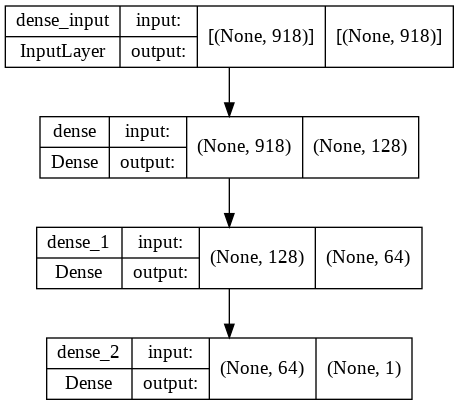
\includegraphics[width=0.6\textwidth, height=0.3\textheight]{nn_arch}
	\caption[Custom Neural Network Architecture]{Custom Neural Network Architecture}
	\label{fig:nn_arch}
\end{figure}

\subsection{Model 7 - \acf{GRU}}
Figure \ref{fig:gru_arch} represents the architecture of the GRU based model for predicting credit card default. The primary dataset is used for training this model;furthermore, the tanh function is used as the activation function and sigmoid  is used as the recurrent activation function  for the GRU layer. Dropout of 10\%, recurrent dropout of 50\% added to reduce the overfitting problem. The output of the GRU layer is then fed to dense layer followed by another dense layer with activation sigmoid for making final prediction. Optimizer used is Adam \& the loss function is Binary Cross Entropy. A dataset generator was created to provide input to the model in chunks, this helped to eliminate the memory issues while training. The final model contains 49165 trainable parameters.\\

\begin{figure}[ht]
	\centering
	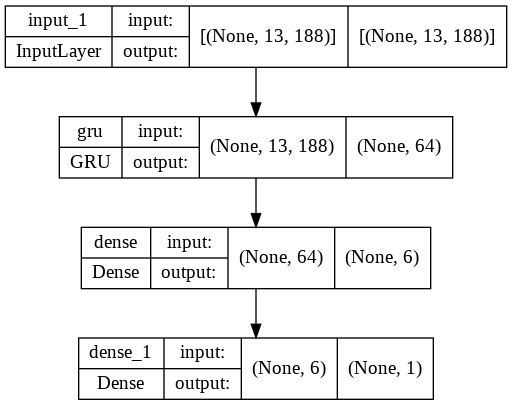
\includegraphics[width=0.6\textwidth, height=0.3\textheight]{gru_arch}
	\caption[GRU Model Architecture]{GRU Model Architecture\\}
	\label{fig:gru_arch}
\end{figure}
\subsection{Model 8 - Ensemble Stacking Model using \acs{ANN} + \acs{GRU} + \acs{GBDT}}
Figure \ref{fig:gru_nn_gbdt_arch} partially depicts the architecture of the custom ensemble stacking model. The primary dataset is first trained using \acs{GRU} layer followed by a dense layer. In parallel, the secondary dataset is trained using a 2 dense layers. Then the output of these two parallel legs were combined to form the concatenation layer. The output of concatenation layer is then trained using a  \acs{GBDT} model to get the final prediction. Adam optimizer was used to optimze the objective binary cross entropy loss function. Instead of loading complete dataset into memory and train the entire dataset in one go, a dataset generator was written to return chunks of data for training, this helped to eliminate the memory overflow issues.\\
\begin{figure}[ht]
	\centering
	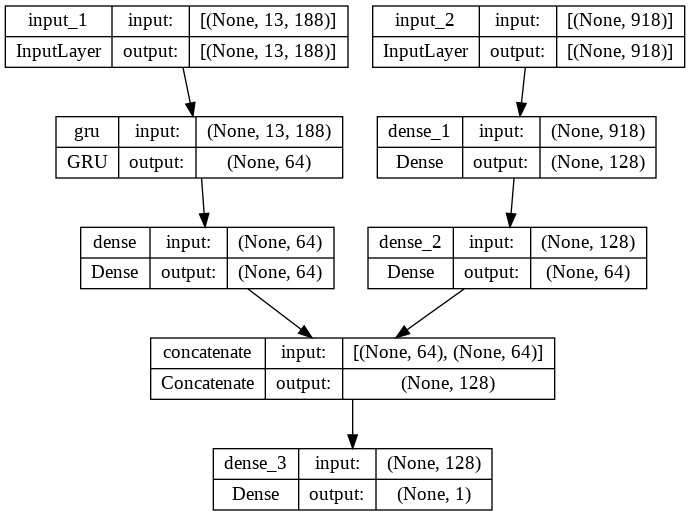
\includegraphics[width=0.7\textwidth, height=0.3\textheight]{GRU_NN_GBDT_Architecture}
	\caption[Custom Ensemble Stacking Model Architecture]{Custom Ensemble Stacking Model Architecture}
	\label{fig:gru_nn_gbdt_arch}
\end{figure}
\subsection{Model 9 - Lean \acs{LGBM} Model}
Finally, a lean model was created using \acs{LGBM} model which peformed on par with the other models but with less resources \& data. Firstly the 20\% of the dataset was set aside as test set and remaining 80\% for training purpose. Training dataset was then oversampled using KMeans \acs{SMOTE} method which resulted in the number of defaulting customers \& non defaulting customers to become equal. Secondly the the training dataset was trained using a simple \acs{SVM} model to extract the feature importances; in addition, the features with feature importance weight less than the mean of importance of weights were discarded. This helped to reduced the feature count from 920 in the secondary dataset to 279. This modified dataset was then passed through a Grid Search CV pipeline to choose the best parameters for maximum depth \& maximum number of leafs for base learner trees, and boosting type. \acf{CV} Recall score was used as the metric to choose the best model. Finally, a \acs{LGBM} model was created using the best model parameters found using GridSearchCV and trained the same on the complete training dataset. The final model was tested and evaluated on the test set.

\subsection{Summary}
Firstly, this section presented overall methodology followed for the experiments followed by the data preprocessing techniques used. Handling of invalid feature values, normalization \& handling memory leakage and memory overflow issue were discussed in the Data Preprocessing section. Secondly, the 9 different models created to solve the problem were discussed. Initially \acs{SVM} model \& Random Forest Classifier model were discussed followed by more advanced machine learning techniques such as \acs{GBDT}, \acs{XGBoost} \& \acs{LGBM}. Then 3 models using deep learning techniques such as Neural Network, \acs{GRU}  and Ensemble Stacking model were presented. Finally a lean model was developed and presented which used less features for training, was computationally less expensive and was explainable model. Before training the final model, the model was passed through a data oversampling pipeline, feature selection pipeline. The model was also tuned using GridSearchCV method to find the optimal hyper parameters. In all the experiments 20\% of data was set aside before training for testing \& evaluation purposes.

\section{Results \& Discussions}\label{sec:results_discussions}

\subsection{Introduction}
Firstly this section presents the test result of the experiments conducted based on the methodology described in section \ref{sec:methodology}. Secondly the main highlights or achievements of the project is discussed. Finally, limitations of this project as well as the future works are discussed.

\subsection{Test Results}
Table \ref{table:results} depicts the result of running the models discussed in section \ref{sec:methodology} on the test set. 4 metrics, F1 Score, Recall, Accuracy \& Precision is used to compare the performance of the models. Though 4 metrics are tracked, Recall \& F1 Score are the metric which is used for Hyper Parameter Tuning, Early Stopping, Cross Validation across all experiments. This decision was taken based on observation that Accuracy will not be a good metric as the dataset is imbalanced; furthermore, the F1 score \& Recall provides a better indictation on how well the model is able to predict the defaulting clients correctly.

\begin{table}[h]
	\begin{center}
		\begin{tabular}{|| c | c | c | c | c ||} 
			\hline
			Model & F1 Score & Recall & Accuracy & Precision \\ [0.5ex] 
			\hline\hline
			SVM	 & 74.66	& 75.57	& 87.24	& \cellcolor[HTML]{ff6666} 73.78 \\
			\hline
			RF	 & \cellcolor[HTML]{ff6666} 73.81	& \cellcolor[HTML]{ff6666} 72.78	& \cellcolor[HTML]{ff6666} 87.13	& 74.86 \\
			\hline
			GBDT	 & 74.33	& 74.13	& 87.25	& 74.52 \\
			\hline
			XGBoost	 & 80.22	& 80.11	& 89.79	& 80.34 \\
			\hline
			LGBM	 & 81.01	& 81.11	& 90.13	& 80.91 \\
			\hline
			ANN	 & \cellcolor[HTML]{339933} 81.03	&  \cellcolor[HTML]{339933} 81.81	& 90.09	& 80.27 \\
			\hline
			GRU	 & 79.81	& 79.96	& 90.67	& 79.65 \\
			\hline
			GRU+ANN+GBDT	 & 80.09	& 79.71	& \cellcolor[HTML]{339933} 90.87	& 80.49 \\
			\hline
			Lean LGBM	 & 80.95	& 80.68	& 90.15	& \cellcolor[HTML]{339933} 81.23 \\
			\hline
		\end{tabular}
		\caption{Comparison of metrics on various models.}
		\label{table:results}
	\end{center}
\end{table}

The \acs{SVM} provided an accuracy of 87.24\% \& F1 score of 74.66 which was impressive considering the model took very less time to train compared to other models; thus, \acs{SVM} model was used in Lean \acs{LGBM} model as part of feature selection pipeline. \acs{RF} model performed worst on F1 Score, Recall \& Accuracy among all the models experimented as part of this project. This reduced performance of \acs{RF} could be due to the large dataset \& dimensionality and the algorithm is not able to generalize well with 100 decision trees. \acs{GBDT} model provided similar results to \acs{SVM} model, however, \acs{GBDT} provided better Precision while \acs{SVM} provided better Recall scores. Ensemble boosting techniques \acs{XGBoost} \& \acs{LGBM} performed really well the test set such that F1 score \& Recall increased almost by  6\% compared to \acs{SVM} model. \acs{LGBM} model performed slightly better than \acs{XGBoost} model in all the metrics and \acs{LGBM} model took less time to train compared to \acs{XGBoost}.

\acs{ANN} model provided the highest F1 Score \& Recall among all the models, however, the difference in F1 Score of \acs{LGBM} and \acs{ANN} model is only 0.02. \acs{ANN}  model provided better Recall score while \acs{LGBM} provided better Precision score. \acs{GRU}+\acs{ANN}+\acs{GBDT} model provided best accuracy score of 90.87 among all the models. \acs{GRU} provided the second best accuracy score;moreover, considering that \acs{GRU} model has 49,165 trainable parameters while the \acs{GRU}+\acs{ANN}+\acs{GBDT} has 178,945, the \acs{GRU} model is able to extract the features better than \acs{GRU}+\acs{ANN}+\acs{GBDT} with less parameters. The table \ref{table:trainable_params} shows the trainable parameter count for the deep learning models explored.

\begin{table}[h]
	\begin{center}
		\begin{tabular}{|| c | c ||} 
			\hline
			Model & Trainable Parameters \\ [0.5ex] 
			\hline\hline
			ANN	& 125,953 \\
			\hline
			GRU	& 49,165 \\
			\hline
			GRU+ANN+GBDT	& 178,945 \\
			\hline
		\end{tabular}
		\caption{Trainable parameters comparison of Deep Learning Models}
		\label{table:trainable_params}
	\end{center}
\end{table}

The Lean \acs{LGBM} model provides a F1 Score of 80.95 which is only 0.08 less than the best performing \acs{ANN} model; futhermore, the Lean \acs{LGBM} provided the best Precision score among all the models. Lean \acs{LGBM} model uses only 1/3rd of the features used by the \acs{ANN} model and still provides comparable performance. The figure \ref{fig:cm_ml} represents the confusion matrix of all the Machine Learning models explored during this project.

\begin{figure}[h!]
	
	\begin{subfigure}{0.4 \textwidth}
		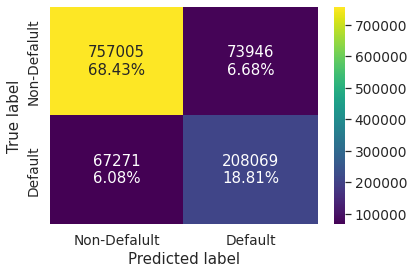
\includegraphics[width=1\linewidth, height=0.8\linewidth]{cm_svm}
		\subcaption[Support Vector Machine]{\acs{SVM}}
		\label{fig:cm_svm}
	\end{subfigure}
	\hfill
	\begin{subfigure}{0.4 \textwidth}
		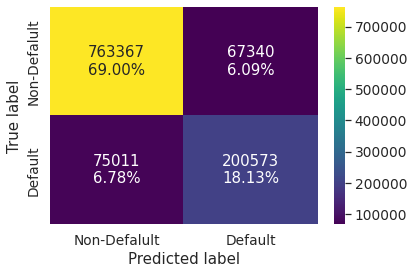
\includegraphics[width=1\linewidth, height=0.8\linewidth]{cm_rf}
		\caption[Random Forest]{\acs{RF}}
		\label{fig:cm_rf}
	\end{subfigure}
	\begin{subfigure}{0.4 \textwidth}
		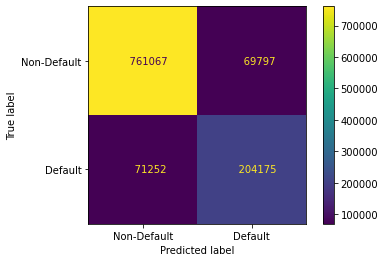
\includegraphics[width=1\linewidth, height=0.8\linewidth]{cm_gbdt}
		\caption[Gradient Boosting Decision Tree]{\acs{GBDT}}
		\label{fig:cm_gbdt}
	\end{subfigure}
	\hfill
	\begin{subfigure}{0.4 \textwidth}
		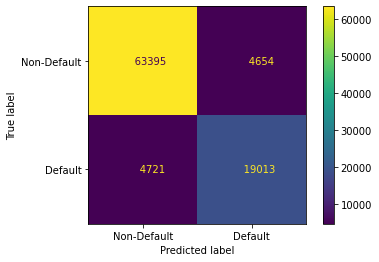
\includegraphics[width=1\linewidth, height=0.8\linewidth]{cm_xgboost}
		\caption[Xtreme Gradient Boosting Descision Tree]{\acs{XGBoost}}
		\label{fig:cm_xgboost}
	\end{subfigure}
	\begin{subfigure}{0.4 \textwidth}
		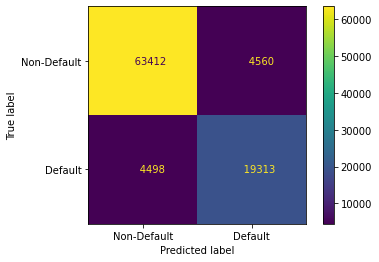
\includegraphics[width=1\linewidth, height=0.8\linewidth]{cm_lgbm}
		\caption[Light Gradient Boosting Machine]{\acs{LGBM}}
		\label{fig:cm_lgbm}
	\end{subfigure}
	\hfill
		\begin{subfigure}{0.4 \textwidth}
		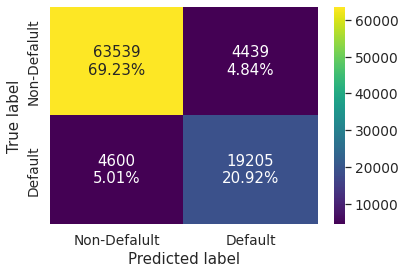
\includegraphics[width=1\linewidth, height=0.8\linewidth]{cm_lean_lgbm}
		\caption[Lean Light Gradient Boosting Machine]{Lean LGBM}
		\label{fig:cm_lean_lgbm}
	\end{subfigure}
	\caption[Confusion Matrix of Machine Leaning Models]{Confusion Matrix of Machine Leaning Models}
	\label{fig:cm_ml}
\end{figure}
\subsubsection{Feature Importance} \label{subsec:feature_imp}
The table \ref{table:imp_features} represents the top 5 features based on the importance from model Lean \acs{LGBM}. This is another advantage of Lean \acs{LGBM} model over the \acs{ANN} model, the Lean \acs{LGBM} model is explainable. However, the features in the Primary Dataset \& Secondary Dataset is anonymized, hence it is not possible to know the exact real life meaning of these features.

\begin{table}[h]
	\begin{center}
		\begin{tabular}{|| c | c ||} 
			\hline
			Feature & Importance Score \\ [0.5ex] 
			\hline\hline
			D\_39\_last &	226 \\
			\hline
			P\_2\_last &	214 \\
			\hline
			B\_4\_last &	191 \\
			\hline
			B\_3\_last &	162 \\
			\hline
			B\_1\_last &	144 \\
			\hline
		\end{tabular}
		\caption{Important Features Extracted Based on Lean \acs{LGBM} model  (Secondary Dataset)}
		\label{table:imp_features}
	\end{center}
\end{table}


\subsection{Achievements}
As mentioned in \ref{sec:literature_review}, most of the previous work on credit card default prediction was based on dataset containing records less than 100,000. However the Primary Dataset used in this work has around 5 Million records of 400,000 unique customers. Most of the previous works concluded that the Ensemble Boosting classifier such as \acs{XGBoost} \& \acs{GBDT} performed better than the traditional machine learning algorithms, this is reconfirmed on large dataset with the work of this project. On the other hand, this work helped to identify  that the difference in peformances between the Deep Learning Network \& Ensemble Boosting Algorithms reduced on large dataset, however it the differences were significant in the smaller datasets. Finally, it was reconfirmed that the models performed better on balanced data and  KMeans \acs{SMOTE} is a suitable candidate for fixing the class imbalance.

\subsection{Limitations \& Future Work}

\subsubsection{Limitations}
Training using some of the traditional machine learning algorithms, such as Non Linear \acs{SVM}, \acf{KNN} etc, were not possible due to the large dataset size and the related time complexity. Feature selection using Sequential Feature Selection technique was tried to select 50 features from the Secondary Dataset;however, due to the large number of features and the large dataset size, Sequential Feature Selection did not complete even after 20 hours. Thus, due to the time constraint on the project as well as the cost related to training on Google Colab, Sequential Feature Selection was dropped from experiments and instead Select From Model technique were used.

Additionally, though multiple data over/under sampling techniques, such as SVMSMOTE, BorderlineSMOTE, Cluster Centroids etc,  were tried, none of them worked as some throw memory overflow issue and others did not complete due to higher time complexity. Since the features of the dataset is anonymized, applying domain knowledge to feature selection process was not possible; moreover, features identified as important in section \ref{subsec:feature_imp} can not be made sense in real life as the features are anonymized. 
Finally, the  data types auto-detected by the Pandas framework while loading dataset is not optimal because even though some of the features contains values between 0 - 1 with precision up to 10 decimal points, still Pandas chooses float64 as the datatype by default. This causes the in memory size of the dataset to quickly exceed the available memory and making impossible to try some of the machine learning algorithms.

\subsubsection{Future Work}
Scikit Learn \citep{scikit-learn} provides limited support for parallel computing, yet this can be explored to make certain computations faster and it might help to overcome some of the computation related limitations mentioned in previous section. Since the data types auto-detected by the Pandas framework while loading dataset is not optimal, one can explore individual features and manually find an optimal datatype of the feature and save this new dataset in parquet format. This will help to reduce the overall size of the dataset and will make loading the dataset to memory much easier.

Attention based Transformer networks recently shown to perform well for time series based classification tasks \citep{wen2022transformers}, \citep{lim2021temporal}, \citep{cholakov2021transformers}, this could be explored on the Primary Dataset to extract dynamic features or could be used as part of the Ensemble Stacking model as one of the learners. TabNet (Attentive Interpretable Tabular Learning)\citep{arik2021tabnet} architecture on classification problems with tabular dataset provides promising performance;thus, this architecture could be explored on the Primary/Secondary dataset to check if provides better performance than the models explored in this project.

In order to overcome some of the challenges related to feature selection mentioned in the previous section, one can explore the idea of stacking the different feature selection techniques in sequential manner, so that less expensive feature selection technique is applied first and then more expensive techniques applied later in the feature selection pipeline.
\subsection{Summary}
In summary, this section initially discussed the evaluation results of different model on the test set. It was identified that the \acs{ANN} network scored the highest on F1 Score \& Recall metrics while \acs{GRU}+\acs{ANN}+\acs{GBDT} scored the highest score on accuracy metric. The Lean \acs{LGBM} model performed on par with the best scoring models while using less features;also, the Lean \acs{LGBM} scored highest on Precision metrics. Top 5 important features were identified from the Lean \acs{LGBM} model result and the same was presented.
Then the achievements of the experiments, such as reconfirming understanding from prior studies on huge industry scale dataset and identifying that the performance of Ensemble Boosting models is on par with the deep learning architecture performance on large datasets.
Finally, the limitations related to the data sampling, feature selection, huge dataset size were discussed along with proposing future works that could be conducted on the dataset \& models.

\section{Conclusion}\label{sec:conclusion}
The objective of this project was to explore different machine learning algorithms \& deep learning architectures on the American Express default prediction dataset\citep{amex-default-prediction-dataset} to predict if a customer will default on the payment in the future. 8 different models (5 Machine Learning \& 3 Deep Learning models) were explored in this project;subsequently, it was identified that \acf{ANN} networks performed best in terms of F1 Score metrics. However, \acs{ANN} model only performed slightly better then the best performing machine learning model, \acs{LGBM};more importantly, the increase in performance was almost negligible considering the complexity of deep learning networks to traditional machine learning models and the non-explainability of \acs{ANN} models.Thus, we can conclude that the \acs{LGBM} is a better choice for credit card default prediction in a industry environment, this is because the explainability of Machine Learning model could become useful for the organizations which require to provide explanations regarding the model to Regulatory Authorities.

Based on the above conclusion, an improved \& efficient model, Lean \acs{LGBM}, was proposed which uses 1/3rd of the features ( hence less dataset size) of the Secondary Dataset to provide performance on par with the \acs{LGBM} \& \acs{ANN} models. This Lean \acs{LGBM} model uses Feature Selection Techniques, Data Oversampling Technique(KMeans-\acs{SMOTE}) and Hyper Parameter tuning to obtain high performance with minimal computations. 

In conclusion,   as reported in various studies \citep{alam2020investigation}, \citep{faraj2021comparison}, \citep{emil2019enhancing}, the Ensemble Boosting techniques such as \acs{XGBoost} \& \acs{LGBM} provides best performance in terms of F1 Score \& computation for credit card default prediction problems. 



\vfill
\clearpage
\lhead{}\chead{MSc. Project Report :: \nouppercase{\leftmark}}\rhead{}
\phantomsection
\addcontentsline{toc}{section}{References}
\bibliographystyle{agsm} 
\bibliography{mybib}

\vfill
\clearpage
\section{Appendix One: Code}

\subsection{Directory Structure} 

\subsection{Running the Provided Code}

\clearpage
\end{document}


